\chapter{Sistemas de ecuaciones lineales\\ Linear equation systems}\index{sistemas} \index[eng]{systems}
\chaptermark{Sistemas \textreferencemark\ Systems}
\epigraph{Después de cada guerra \\ alguien tiene que limpiar. \\ No se van a ordenar solas las cosas, \\ digo yo. (Maria Wisława Anna Szymborska)}

\begin{paracol}{2}

\section{Introducción}

Una ecuación lineal es aquella que establece una relación \emph{lineal} entre dos o más variables, por ejemplo,

\begin{equation*}
3x_1-2x_2=12
\end{equation*}

Se dice que es una relación lineal, porque las variables están relacionadas entre sí tan solo mediante sumas y productos por coeficientes constantes. En particular, el ejemplo anterior puede representarse geométricamente mediante una línea recta.

El número de variables relacionadas en una ecuación lineal determina la dimensión de la ecuación. La del ejemplo anterior es una ecuación bidimensional, puesto que hay dos variables. El número puede ser arbitrariamente grande en general,
\begin{equation*}
a_1x_1+a_2x_2+\cdots +a_nx_n=b
\end{equation*} 
será una ecuación n-dimensional.

\switchcolumn    

\section{Introduction}

A linear equation is an equation that establishes a \emph{linear} relationship between two or more variables, for example,

\begin{equation}
3x_1-2x_2=12
\end{equation}

It is said to be a linear relationship, because the variables are related to each other only through additions and products by constant coefficients. In particular, the above example can be represented geometrically by a straight line.

The number of related variables in a linear equation determines the dimension of the equation. The above example is a two-dimensional equation, since there are two variables. The number can be arbitrarily large in general,
\begin{equation*}
a_1x_1+a_2x_2+cdots +a_nx_n=b
\end{equation*} 
will be an n-dimensional equation.

\switchcolumn
Como ya hemos señalado más arriba, una ecuación bidimensional admite una línea recta como representación geométrica, una ecuación tridimensional admitirá un plano y para dimensiones mayores que tres cada ecuación representará un hiperplano de dimension n. Por supuesto, para dimensiones mayores que tres, no es posible obtener una representación gráfica de la ecuación.

Las ecuaciones lineales juegan un papel muy importante en la física y, en general en la ciencia y la tecnología. La razón es que constituyen la aproximación matemática más sencilla a la relación entre magnitudes físicas. Por ejemplo cuando decimos que la fuerza aplicada a un resorte y la elongación  que sufre están relacionadas por la ley de Hooke, $F=Kx$ estamos estableciendo una relación lineal entre las magnitudes fuerza y elongación. ¿Se cumple siempre dicha relación? Desde luego que no. Pero es razonablemente cierta para elongaciones pequeñas y, apoyados en ese sencillo modelo \emph{lineal} de la realidad, se puede aprender mucha física.

Un sistema de ecuaciones lineales está constituido por varias ecuaciones lineales, que expresan relaciones lineales distintas sobre las mismas variables. Por ejemplo,

\begin{align*}
a_{11}x_1+a_{12}x_2&=b_1\\
a_{21}x_1+a_{22}x_2&=b_2
\end{align*}

\switchcolumn
As we have already pointed out above, a two-dimensional equation admits a straight line as geometrical representation, a three-\-di\-men\-sio\-nal equation will admit a plane and for dimensions greater than three each equation will represent a hyperplane of dimension n. Of course, for dimensions greater than three, it is not possible to obtain a graphical representation of the equation.

Linear equations play a very important role in physics and, in general, in science and technology. The reason is that they are the simplest mathematical approximation of the relationship between physical quantities. For example, when we say that the force applied to a spring and the elongation it undergoes are related by Hooke's law, $F=Kx$, we are establishing a linear relationship between the quantities force and elongation. Does this relationship always hold true? Certainly not. But it is reasonably true for small elongations and, based on this simple \emph{linear} model of reality, a lot of physics can be learned.

A system of linear equations is made up of several linear equations, which express different linear relationships about the same variables. For example,

\begin{align*}
a_{11}x_1+a_{12}x_2&=b_1\\
a_{21}x_1+a_{22}x_2&=b_2
\end{align*}

\switchcolumn

Se llaman soluciones del sistema de ecuaciones a los valores de las variables que satisfacen simultáneamente a todas las ecuaciones que componen el sistema. Desde el punto de vista de la obtención de las soluciones a las variables se les suele denominar incógnitas, es decir valores no conocidos que deseamos obtener o calcular.

Un sistema de ecuaciones puede tener infinitas soluciones, puede tener una única solución o puede no tener solución. En lo que sigue, nos centraremos en sistemas de ecuaciones que tienen una única solución. 

Una primera condición para que un sistema de ecuaciones tengan una única solución es que el número de incógnitas presentes en el sistema coincida con el número de ecuaciones. 

\switchcolumn

The values of the variables that simultaneously satisfy all the equations that make up the system are called solutions of the system of equations. From the point of view of obtaining the solutions, the variables are usually called unknowns, i.e. unknown values that we wish to obtain or calculate.

A system of equations can have infinite solutions, it can have only one solution or it can have no solution. In what follows, we will focus on systems of equations that have only one solution. 

A first condition for a system of equations to have a unique solution is that the number of unknowns present in the system coincides with the number of equations. 

\switchcolumn

De modo general podemos decir que vamos a estudiar métodos numéricos para resolver con un computador sistemas de $n$ ecuaciones con $n$ incógnitas,

\begin{align*}
a_{11}&x_1+a_{12}x_2+\cdots +a_{1n}x_n=b_1\\
a_{21}&x_1+a_{22}x_2+\cdots +a_{2n}x_n=b_2\\
\cdots & \\
a_{n1}&x_1+a_{n2}x_2+\cdots +a_{nn}x_n=b_n
\end{align*}  

Una de las grandes ventajas de los sistemas de ecuaciones lineales es que puede expresarse en forma de producto matricial,

\switchcolumn

In general terms, we can say that we are going to study numerical methods to solve with a computer systems of $n$ equations with $n$ unknowns,

\begin{align*}
a_{11}&x_1+a_{12}x_2+\cdots +a_{1n}x_n=b_1\\
a_{21}&x_1+a_{22}x_2+\cdots +a_{2n}x_n=b_2\\
\cdots & \\
a_{n1}&x_1+a_{n2}x_2+\cdots +a_{nn}x_n=b_n
\end{align*}  

One of the great advantages of systems of linear equations is that they can be expressed in matrix product form,

\end{paracol}



\begin{equation*}
\left. \begin{aligned}
a_{11}&x_1+a_{12}x_2+\cdots +a_{1n}x_n=b_1\\
a_{21}&x_1+a_{22}x_2+\cdots +a_{2n}x_n=b_2\\
\cdots & \\
a_{n1}&x_1+a_{n2}x_2+\cdots +a_{nn}x_n=b_n
\end{aligned}\right\} \Rightarrow	\overbrace{\begin{pmatrix}
a_{11}& a_{12}& \cdots & a_{1n}\\
a_{21}& a_{22}& \cdots & a_{2n}\\
\vdots & \vdots & \ddots & \vdots\\
a_{n1}& a_{n2}& \cdots & a_{nn}
\end{pmatrix}}^A \cdot \overbrace{\begin{pmatrix}
x_1\\
x_2\\
\vdots \\
x_n
\end{pmatrix}}^x=\overbrace{\begin{pmatrix}
b_1\\
b_2\\
\vdots \\
b_n
\end{pmatrix}}^b
\end{equation*}

\begin{paracol}{2}
    La matriz $A$ recibe el nombre de matriz de coeficientes del sistema de ecuaciones, el vector $x$ es el vector de incógnitas y el vector $b$ es el vector de términos independientes. Para resolver un sistema de ecuaciones podríamos aplicar álgebra de matrices, como se ha visto en el capítulo \ref{ch:numpy}:
    
\switchcolumn
    The matrix $A$ is called the coefficient matrix of the system of equations, the vector $x$ is the vector of unknowns and the vector $b$ is the vector of independent terms. To solve a system of equations we could apply matrix algebra, as discussed in chapter \ref{ch:numpy}:
    
\end{paracol}

\begin{equation*}
A\cdot x=b \Rightarrow x=A^{-1}\cdot b
\end{equation*}

\begin{paracol}{2}
Es decir, bastaría invertir la matriz de coeficientes y multiplicarla por la izquierda por el vector de coeficientes para obtener el vector de  términos independientes. De aquí podemos deducir una segunda condición para que un sistema de ecuaciones tenga una solución única; Su matriz de coeficientes tiene que tener inversa. Veamos algunos ejemplos sencillos.

Tomaremos en primer lugar un sistema de dos ecuaciones con dos incógnitas,

\begin{align*}
4x_1+x_2&=6\\
3x_1-2x_2&=-1
\end{align*}

Si expresamos el sistema en forma de producto de matrices obtenemos,

\switchcolumn

That is, it would be enough to invert the matrix of coefficients and multiply it on the left by the vector of coefficients to obtain the vector of independent terms. From this we can deduce a second condition for a system of equations to have a unique solution; its coefficient matrix must have an inverse. Let us look at some simple examples.

We will first take a system of two equations with two unknowns,

\begin{align*}
4x_1+x_2&=6 \\
3x_1-2x_2&=-1
\end{align*}

If we express the system as a product of matrices we obtain,

\end{paracol}

\begin{equation*}
\begin{pmatrix}
4& 1\\
3& -2
\end{pmatrix} \cdot \begin{pmatrix}
x_1\\
x_2
\end{pmatrix}=\begin{pmatrix}
6\\
-1
\end{pmatrix}
\end{equation*}

\begin{paracol}{2}
e invirtiendo la matriz de coeficientes y multiplicándola por el vector de términos independientes se llega al vector de soluciones del sistema,

\switchcolumn
and by inverting the coefficient matrix and multiplying it by the vector of independent terms we arrive at the vector of solutions of the system,

\end{paracol}

\begin{equation*}
\begin{pmatrix}
x_1\\
x_2
\end{pmatrix}= \begin{pmatrix}
4& 1\\
3& -2
\end{pmatrix}^{-1} \cdot \begin{pmatrix}
6\\
-1
\end{pmatrix}=\begin{pmatrix}
2/11& 1/11\\
3/11& -4/11
\end{pmatrix}\begin{pmatrix}
6\\
-1
\end{pmatrix}=\begin{pmatrix}
1\\
2
\end{pmatrix}
\end{equation*}

\begin{paracol}{2}
En el ejemplo que acabamos de ver, cada ecuación corresponde a una recta en el plano, en la figura \ref{fig:recta1} se han representado dichas rectas gráficamente. El punto en que se cortan es precisamente la solución del sistema.

\switchcolumn
In the example we have just seen, each equation corresponds to a line in the plane, in the figure \ref{fig:recta1} these lines have been represented graphically. The point where they intersect is precisely the solution of the system.

\end{paracol}
\begin{figure}[h]
\centering
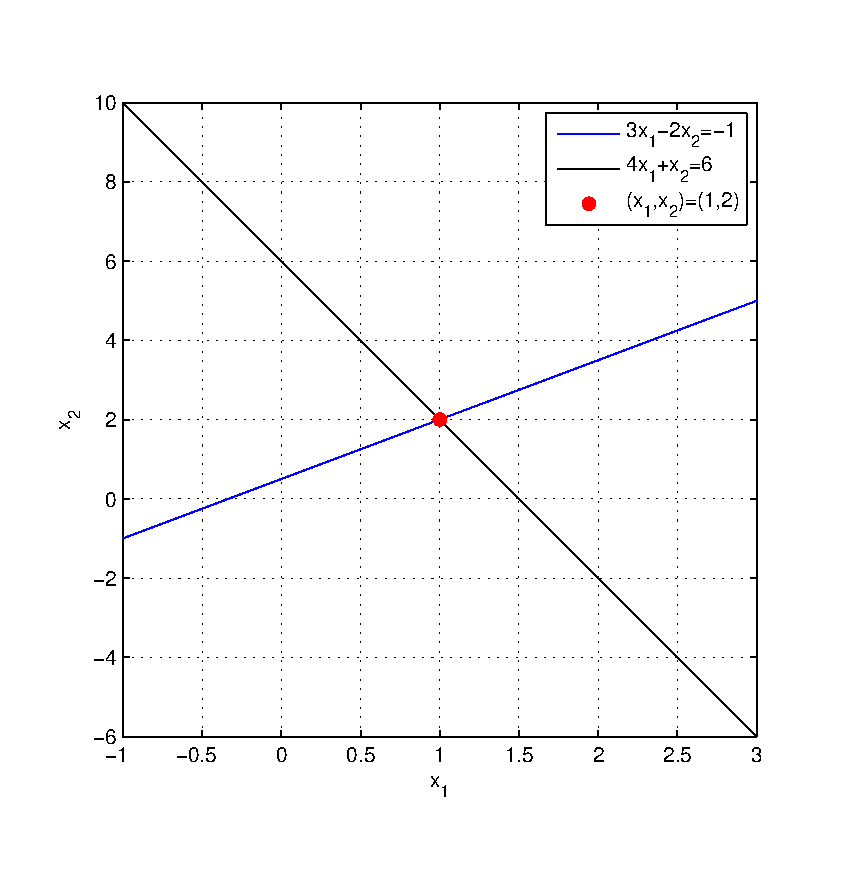
\includegraphics[width=12cm]{recta1}
\bicaption{Sistema de ecuaciones con solución única}{Equation system with unique solution}
\label{fig:recta1}
\end{figure}

\begin{paracol}{2}
    
Supongamos ahora el siguiente sistema, también de dos ecuaciones con dos incógnitas,

\begin{align*}
4x_1+x_2&=6\\
2x_1+\frac{1}{2} x_2&=-1
\end{align*}

El sistema no tiene solución. Su matriz de coeficientes tiene determinante cero, por lo que no es invertible,
\begin{equation*}
\vert A \vert =\begin{vmatrix}
4& 1\\
2& 1/2
\end{vmatrix} =0 \Rightarrow \nexists A^{-1}
\end{equation*}

\switchcolumn
Now suppose the following system, also of two equations with two unknowns,
\begin{align*}
4x_1+x_2&=6\\
2x_1+\frac{1}{2} x_2&=-1
\end{align*}

The system has no solution. Its coefficient matrix has zero determinant, so it is not invertible,
\begin{equation*}
\vert A \vert =\begin{vmatrix}
4& 1\\
2& 1/2
\end{vmatrix} =0 \Rightarrow \nexists A^{-1}
\end{equation*}

\switchcolumn
Si representamos gráficamente las dos ecuaciones de este sistema (figura \ref{fig:recta2}) es fácil entender lo que pasa, las rectas son paralelas, no existe ningún punto $(x_1,x_2)$ que pertenezca a las dos rectas, y por tanto el sistema carece de solución.

\switchcolumn
If we represent graphically the two equations of this system (figure \ref{fig:recta2}) it is easy to understand what happens, the lines are parallel, there is no point $(x_1,x_2)$ that belongs to the two lines, and therefore the system has no solution.

\end{paracol}



\begin{figure}[h]
\centering
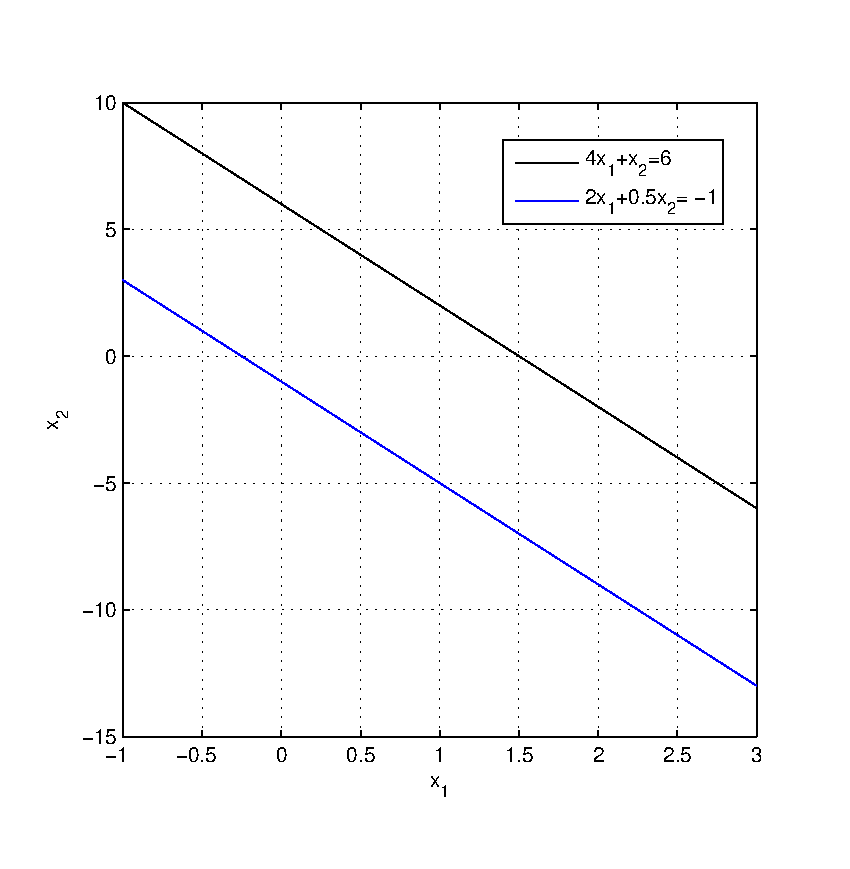
\includegraphics[width=12cm]{recta2}
\bicaption{Sistema de ecuaciones sin solución}{Equation system without solution}
\label{fig:recta2}
\end{figure}

\begin{paracol}{2}
Dos rectas paralelas lo son, porque tienen la misma pendiente. Esto se refleja en la matriz de coeficientes, en que las filas son proporcionales; si multiplicamos la segunda fila por dos, obtenemos la primera. 

\switchcolumn

Two parallel lines are parallel because they have the same slope. This is reflected in the coefficient matrix, where the rows are proportional; if we multiply the second row by two, we get the first row. 

\switchcolumn
Por último, el sistema,

\begin{align*}
4x_1+x_2&=6\\
2x_1+\frac{1}{2} x_2&=3
\end{align*}

posee infinitas soluciones. La razón es que la segunda ecuación es igual que la primera multiplicada por dos: es decir, representa exactamente la misma relación lineal entre las variables $x_1$ y $x_2$, por tanto, todos los puntos de la recta son solución del sistema. De nuevo, la matriz de coeficientes del sistema no tiene inversa ya que su determinante es cero.

\switchcolumn
Finally, the system,

\begin{align*}
4x_1+x_2&=6 \\
2x_1+\frac{1}{2} x_2&=3
\end{align*}

has infinite solutions. The reason is that the second equation is the same as the first equation multiplied by two: that is, it represents exactly the same linear relationship between the variables $x_1$ and $x_2$, therefore, all the points on the line are solutions of the system. Again, the coefficient matrix of the system has no inverse since its determinant is zero.
\end{paracol}

\begin{figure}[h]
\centering
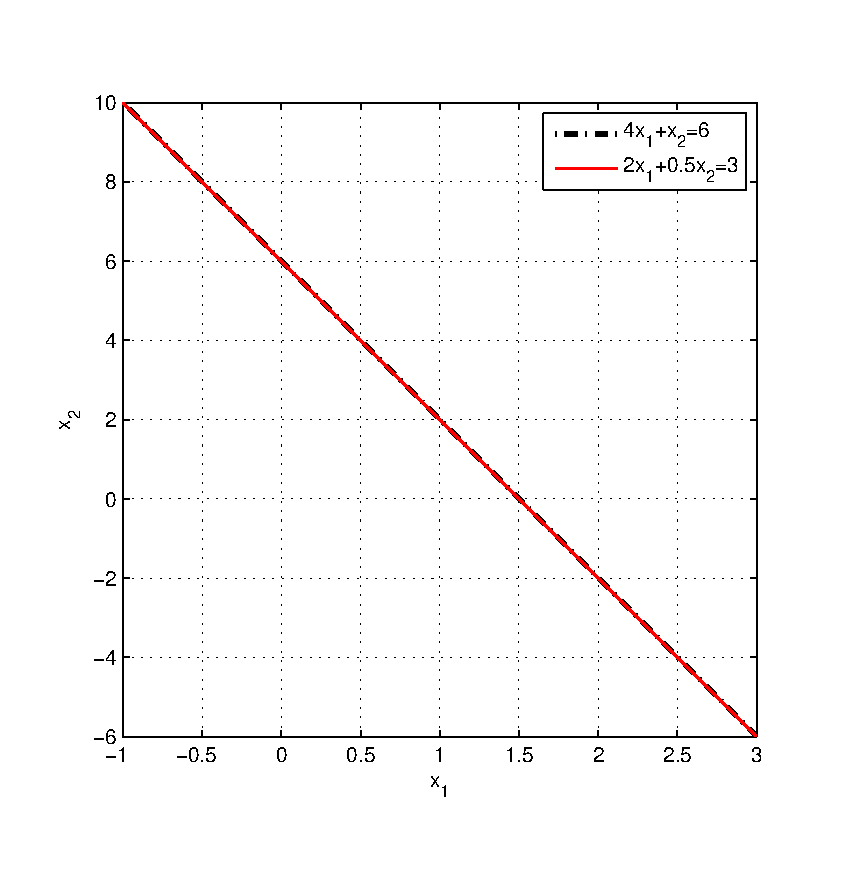
\includegraphics[width=12cm]{recta3.eps}
\bicaption{Sistema de ecuaciones con infinitas soluciones}{Equation system with infinite solutions}
\label{recta3}
\end{figure}

\begin{paracol}{2}
Para sistemas de ecuaciones de dimensión mayor, se cumple también que que el sistema no tiene solución única si el determinante de su matriz de coeficiente es cero. En todos los demás casos, es posible obtener la solución del sistema invirtiendo la matriz de coeficientes y multiplicando el resultado por el vector de términos independientes.

En cuanto un sistema de ecuaciones tiene una dimensión suficientemente grande, invertir su matriz de coeficientes se torna un problema costoso o sencillamente inabordable.

Desde un punto de vista numérico, la inversión de una matriz, presenta frecuentemente problemas debido al error de redondeo en las operaciones. Por esto, casi nunca se resuelven los sistemas de ecuaciones invirtiendo su matriz de coeficientes. A lo largo de este capítulo estudiaremos dos tipos de métodos de resolución de sistemas de ecuaciones. El primero de ellos recibe el nombre genérico de métodos directos, el segundo tipo lo constituyen los llamados métodos iterativos.

\switchcolumn
For higher dimensional systems of equations, it is also true that the system has no unique solution if the determinant of its coefficient matrix is zero. In all other cases, it is possible to obtain the solution of the system by inverting the coefficient matrix and multiplying the result by the vector of independent terms.

As soon as a system of equations has a sufficiently large dimension, inverting its coefficient matrix becomes a costly or simply intractable problem.

From a numerical point of view, the inversion of a matrix often presents problems due to the rounding error in the operations. For this reason, systems of equations are almost never solved by inverting their matrix of coefficients. Throughout this chapter we will study two types of methods for solving systems of equations. The first of these is known generically as direct methods, while the second type is known as iterative methods.

\switchcolumn
\section{Condicionamiento}
En la introducción hemos visto que para que un sistema de ecuaciones tenga solución, es preciso que su matriz de coeficientes sea invertible. Sin embargo cuando tratamos de resolver un sistema de ecuaciones numéricamente, empleando un ordenador, debemos antes examinar cuidadosamente la matriz de coeficientes del sistema. Veamos un ejemplo: el sistema,

\begin{align*}
4x_1+x_2&=6\\
2x_1+0.4 x_2&=-1
\end{align*}

\switchcolumn
\section{Condition number}
In the introduction we have seen that for a system of equations to have a solution, its coefficient matrix must be invertible. However, when we try to solve a system of equations numerically, using a computer, we must first carefully examine the matrix of coefficients of the system. Let us look at an example: the system,

\begin{align*}
4x_1+x_2&=6\\
2x_1+0.4 x_2&=-1
\end{align*}

\switchcolumn

Tiene como soluciones,
\begin{equation*}
x=\begin{pmatrix}
-8.5\\
40
\end{pmatrix}
\end{equation*}

\switchcolumn
 Has the following solutions,
 \begin{equation*}
x=\begin{pmatrix}
-8.5\\
40
\end{pmatrix}
\end{equation*}

\switchcolumn

Si alteramos ligeramente uno de sus coeficientes,

\begin{align*}
4x_1+x_2&=6\\
2x_1+0.4{\color{red}9} x_2&=-1
\end{align*}

\switchcolumn

If we slightly change one of the coefficients,
\begin{align*}
4x_1+x_2&=6\\
2x_1+0.4{\color{red}9} x_2&=-1
\end{align*}

\switchcolumn

Las soluciones se alteran bastante;  se vuelven aproximadamente 10 veces más grande,
\begin{equation*}
x=\begin{pmatrix}
-98.5\\
400
\end{pmatrix}
\end{equation*}

\switchcolumn

The solutions become quite altered; they become about 10 times larger,
\begin{equation*}
x=\begin{pmatrix}
-98.5\\
400
\end{pmatrix}
\end{equation*}

\switchcolumn
y si volvemos a alterar el mismo coeficiente,

\begin{align*}
4x_1+x_2&=6\\
2x_1+0.4{\color{red}99} x_2&=-1
\end{align*}

\switchcolumn

if we change again the same coefficient,

\begin{align*}
4x_1+x_2&=6\\
2x_1+0.4{\color{red}99} x_2&=-1
\end{align*}

\switchcolumn

La solución es aproximadamente 100 veces más grande,
\begin{equation*}
x=\begin{pmatrix}
-998.5\\
4000
\end{pmatrix}
\end{equation*}

\switchcolumn

The solution is about 100 times larger,

\begin{equation*}
x=\begin{pmatrix}
-998.5\\
4000
\end{pmatrix}
\end{equation*}

\switchcolumn
La razón para estos cambios es fácil de comprender intuitivamente; a medida que aproximamos el coeficiente a $0.5$, estamos haciendo que las dos ecuaciones lineales sean cada vez mas paralelas, pequeñas variaciones en la pendiente, modifican mucho la posición del punto de corte.

Cuando pequeñas variaciones en la matriz de coeficientes generan grandes variaciones en las soluciones del sistema, se dice que el sistema está mal condicionado, en otras palabras: que no es un sistema bueno para ser resuelto numéricamente. Las soluciones obtenidas para un sistema mal condicionado, hay que tomarlas siempre con bastante escepticismo.

Para estimar el buen o mal condicionamiento de un sistema, se emplea el número de condición, que definimos en el capítulo \ref{ch:numpy} en la sección \ref{sec:SVD}, al hablar de la factorización SVD. El número de condición de una matriz es el cociente entre sus valores singulares mayor y menor.  Cuanto más próximo a $1$ sea el número de condición, mejor condicionada estará la matriz y cuanto mayor sea el número de condición peor condicionada estará.

\switchcolumn
The reason for these changes is easy to understand intuitively; as we bring the coefficient closer to $0.5$, we are making the two linear equations more and more parallel, and small variations in the slope greatly modify the position of the cut-off point.

When small variations in the matrix of coefficients generate large variations in the solutions of the system, it is said that the system is ill-conditioned, in other words: that it is not a good system to be solved numerically. The solutions obtained for an ill-conditioned system must always be taken with considerable scepticism.

To estimate the good or bad conditioning of a system, we use the condition number, which we defined in the chapter \ref{ch:numpy} in section \ref{sec:SVD}, when talking about SVD factorisation. The condition number of a matrix is the quotient of its largest and smallest singular values.  The closer the condition number is to $1$, the better conditioned the matrix is, and the larger the condition number, the worse conditioned it is.

\switchcolumn

En Python dentro del paquete \texttt{linalg} de \texttt{numpy} está la función \texttt{cond} que nos permite obtener el número de condición de una matriz. Si lo aplicamos a la matriz de coeficientes del último ejemplo mostrado,

\switchcolumn
In Python, we can use the function \texttt{cond} inside the \texttt{linalg} module in \texttt{numpy} to compute the condition number of a matrix. We can apply to the last example coefficient matrix

\end{paracol}

\begin{minted}{pycon}
import numpy as np

A=np.array([[4,1],[2,0.499]])

np.linalg.cond(A)
Out[7]: 5312.250061755533
\end{minted}

\begin{paracol}{2}
El número está bastante alejado de uno, lo que, en principio, indica un mal condicionamiento del sistema. 

Incidentalmente, podemos calcular la factorización svd de la matriz de coeficientes y dividir el valor singular mayor entre el menor para comprobar que el resultado es el mismo que nos da la función \texttt{cond},

\switchcolumn
The number is quite far from one, which, in principle, indicates a ill-condition of the system. 

Incidentally, we can calculate the factorisation svd of the coefficient matrix and divide the largest singular value by the smallest to check that the result is the same as that given by the function \texttt{cond},
\end{paracol}

\begin{minted}{pycon}
[U,S,Vt]=np.linalg.svd(A)

S[0]/S[1]
Out[14]: 5312.250061755533
\end{minted}

\begin{paracol}{2}
\section{Métodos directos}
\subsection{Sistemas triangulares}
Vamos a empezar el estudio de los métodos directos por los algoritmos de resolución de los sistemas más simples posibles, aquellos cuya matriz de coeficientes es una matriz diagonal, triangular superior o triangular inferior.
\paragraph{Sistemas diagonales.} Un sistema diagonal es aquel cuya matriz de coeficientes es una matriz diagonal. 

\switchcolumn

\subsection{Direct methods}
\subsection{Triangular systems}
We are going to begin the study of direct methods with the algorithms for solving the simplest possible systems, those whose coefficient matrix is a diagonal, upper triangular or lower triangular matrix.
\paragraph{ Diagonal systems.} A diagonal system is one whose coefficient matrix is a diagonal matrix. 
\end{paracol}

\begin{equation*}
\left. \begin{aligned}
a_{11}&x_1=b_1\\
a_{22}&x_2=b_2\\
\cdots & \\
a_{nn}&x_n=b_n
\end{aligned}\right\} \Rightarrow	\overbrace{\begin{pmatrix}
a_{11}& 0& \cdots & 0\\
0& a_{22}& \cdots & 0\\
\vdots & \vdots & \ddots & \vdots\\
0& 0& \cdots & a_{nn}
\end{pmatrix}}^A \cdot \overbrace{\begin{pmatrix}
x_1\\
x_2\\
\vdots \\
x_n
\end{pmatrix}}^x=\overbrace{\begin{pmatrix}
b_1\\
b_2\\
\vdots \\
b_n
\end{pmatrix}}^b
\end{equation*}

\begin{paracol}{2}
Su resolución es trivial, basta dividir cada término independiente por el elemento correspondiente de la diagonal de la matriz de coeficientes,
\begin{equation*}
x_i=\frac{b_i}{a_{ii}}
\end{equation*}

\switchcolumn
Its resolution is trivial, just divide each independent term by the corresponding element of the diagonal of the coefficient matrix,
\begin{equation*}
x_i=\frac{b_i}{a_{ii}}
\end{equation*}

\switchcolumn
Para obtener la solución basta crear en Python un sencillo bucle \texttt{for},

\switchcolumn
To compute the solution it is enough to code a simple \texttt{for} loop,
\end{paracol}

\begin{minted}{python}
import numpy as np

def diag_sys(A,b):
    [f,c]=np.shape(A)
    x=np.zeros([f,1])
    for i in range(f):
        x[i]=b[i]/A[i,i]
    return x
\end{minted}


\begin{paracol}{2}
\paragraph{Sistemas triangulares inferiores: método de sustituciones progresivas.} Un sistema triangular inferior de $n$ ecuaciones con $n$ incógnitas tendrá la forma general,
\switchcolumn
\paragraph{Lower triangular systems: method of progressive substitutions.} A lower triangular system of $n$ equations with $n$ unknowns will have the general form,
\end{paracol}

\begin{equation*}
\left. \begin{aligned}
a_{11}&x_1=b_1\\
a_{21}&x_1+a_{22}x_2=b_2\\
\cdots & \\
a_{n1}&x_1+a_{n2}x_2+\cdots +a_{nn}x_n=b_n
\end{aligned}\right\} \Rightarrow	\overbrace{\begin{pmatrix}
a_{11}& 0& \cdots & 0\\
a_{21}& a_{22}& \cdots & 0\\
\vdots & \vdots & \ddots & \vdots\\
a_{n1}& a_{n2}& \cdots & a_{nn}
\end{pmatrix}}^A \cdot \overbrace{\begin{pmatrix}
x_1\\
x_2\\
\vdots \\
x_n
\end{pmatrix}}^x=\overbrace{\begin{pmatrix}
b_1\\
b_2\\
\vdots \\
b_n
\end{pmatrix}}^b
\end{equation*}

\begin{paracol}{2}
El procedimiento para resolverlo a \emph{mano} es muy sencillo,
despejamos la primera la primera incógnita de la primera ecuación,
\begin{equation*}
x_1=\frac{b_1}{a_{11}}
\end{equation*}
\switchcolumn  
The procedure to solve to \emph{hand} is very simple,
we clear the first unknown from the first equation,
\begin{equation*}
x_1=\frac{b_1}{a_{11}}
\end{equation*}

\switchcolumn
A continuación sustituimos este resultado en la segunda ecuación, y despejamos $x_2$,
\begin{equation*}
x_2=\frac{b_2-a_{21}x_1}{a_{22}}
\end{equation*}

\switchcolumn
Next, we substitute this result in the second equation and clear $x_2$
\begin{equation*}
x_2=\frac{b_2-a_{21}x_1}{a_{22}}
\end{equation*}

\switchcolumn

De cada ecuación vamos obteniendo una componente del vector solución, sustituyendo las soluciones obtenidas en las ecuaciones anteriores, así cuando llegamos a la ecuación $i$,

\begin{equation*}
x_i=\frac{b_i-\sum_{j=1}^{i-1}a_{ij}x_j}{a_{ii}}
\end{equation*}

\switchcolumn
From each equation we obtain a component of the solution vector, substituting the solutions obtained in the previous equations, so when we arrive at the equation $i$,

\begin{equation*}
x_i=\frac{b_i-\sum_{j=1}^{i-1}a_{ij}x_j}{a_{ii}}
\end{equation*}

\switchcolumn
Si repetimos este mismo proceso hasta llegar a la última ecuación del sistema, $n$, habremos obtenido la solución completa.

EL siguiente código calcula la solución de un sistema triangular inferior mediante sustituciones progresivas,

\switchcolumn

If we repeat this same process until we reach the last equation of the system, $n$, we will have obtained the complete solution.

The following code calculates the solution of a lower triangular system by progressive substitutions,
\end{paracol}

\begin{minted}{python}
import numpy as np

def progressive(A,b):
    ''' This function computes the solution of a lower equation system using 
    progressive substitution. It receives the coefficient matriz A and the 
    independent term vector b. It returns the vector solution x
    '''
    # Coefficient matrix size. Return error if not square
    [f,c]=np.shape(A)
    if f!=c:
        print("A is not square")
        return
    # To build the solution vector x
    x=np.zeros(f)
    x=b.copy()
    for i in range(f):
        '''The inner block subtracts to the independent term the previous solution
         multiplied by the correspondent coefficient'''
        for j in range(0,i):
            x[i]-=x[j]*A[i,j]
        '''Finaly divide the result by the diagonal coefficient'''
        x[i]=(x[i])/A[i,i]
    return x
\end{minted}

\begin{paracol}{2}


\paragraph{Sistemas triangulares superiores: método de sustituciones regresivas.} En este caso, el sistema general de $n$ ecuaciones con $n$ incógnitas tendrá la forma general,

\switchcolumn
\paragraph{Upper triangular systems: method of backward substitutions.} In this case, the general system of $n$ equations with $n$ unknowns will have the general form,
\end{paracol}

\begin{equation*}
\left. \begin{aligned}
a_{11}x_1+a_{12}x_2+\cdots +a_{1n}x_n=b_1\\
a_{22}x_2+\cdots +a_{2n}x_n=b_2\\
\cdots  \\
a_{nn}x_n=b_n
\end{aligned}\right\} \Rightarrow	\overbrace{\begin{pmatrix}
a_{11}& a_{12}& \cdots & a_{1n}\\
0& a_{22}& \cdots & a_{2n}\\
\vdots & \vdots & \ddots & \vdots\\
0& 0& \cdots & a_{nn}
\end{pmatrix}}^A \cdot \overbrace{\begin{pmatrix}
x_1\\
x_2\\
\vdots \\
x_n
\end{pmatrix}}^x=\overbrace{\begin{pmatrix}
b_1\\
b_2\\
\vdots \\
b_n
\end{pmatrix}}^b
\end{equation*}

\begin{paracol}{2}
    El método de resolución es idéntico al de un sistema triangular inferior, simplemente que ahora, empezamos a resolver por la última ecuación,
\begin{equation*}
x_n=\frac{b_n}{a_{nn}}
\end{equation*}
Y seguimos sustituyendo hacia arriba,
\begin{equation*}
x_{n-1}=\frac{b_{n-1}-a_{(n-1)n}x_{n}}{a_{(n-1)(n-1)}}
\end{equation*}

\begin{equation*}
x_i=\frac{b_i-\sum_{j=i+1}^{n}a_{ij}x_j}{a_{ii}}
\end{equation*}

\switchcolumn
  The method of solution is identical to that of a lower triangular system, except that now, we start solving for the last equation,
\begin{equation*}
x_n=\frac{b_n}{a_{nn}}
\end{equation*}
And we keep substituting upwards,
\begin{equation*}
x_{n-1}=\frac{b_{n-1}-a_{(n-1)n}x_{n}}{a_{(n-1)(n-1)}}
\end{equation*}

\begin{equation*}
x_i=\frac{b_i-\sum_{j=i+1}^{n}a_{ij}x_j}{a_{ii}}
\end{equation*}

\switchcolumn

El código para implementar este método es similar al de las sustituciones progresivas. Se deja como ejercicio el construir una función en Python que calcule la solución de un sistema triangular superior por el método de las sustituciones regresivas.

\switchcolumn
The code to implement this method is similar to that of forward substitutions. It is left as an exercise to build a Python function that calculates the solution of an upper triangular system by the method of backward substitutions.
\switchcolumn
\subsection{Métodos basados en las factorizaciones}
Puesto que sabemos como resolver sistemas triangulares, una manera de resolver sistemas más complejos sería encontrar métodos para reducirlos a sistemas triangulares. De este modo evitamos invertir la matriz de coeficientes y los posibles problemas de estabilidad numérica derivados de dicha operación. Si podemos expresar la matriz $A$ como el producto de matrices diagonales o triangulares podremos resolver el sistema usando los métodos anteriores. \textbf{Factorizar} una matriz es descomponer la misma en el producto de dos o más matrices de alguna forma canónica.

\switchcolumn
\subsection{Methods based on factorisations}

Since we know how to solve triangular systems, one way to solve more complex systems would be to find methods to reduce them to triangular systems. In this way we avoid inverting the matrix of coefficients and the possible problems of numerical stability derived from such an operation. If we can express the matrix $A$ as the product of diagonal or triangular matrices we can solve the system using the above methods. \textbf{To factorise} a matrix is to decompose it into the product of two or more matrices of some canonical form.

\switchcolumn
\paragraph{Factorización LU.} La factorización LU consiste en factorizar una matriz en el producto de dos, una triangular inferior $L$ y una triangular superior $U$. La factorización podía incluir pivoteo de filas, para alcanzar una solución numéricamente estable. En este caso la factorización LU toma la forma,
\begin{equation*}
P\cdot A = L\cdot U
\end{equation*}

Donde $P$ representa una matriz de permutaciones.

Podemos verlo también de otra manera, $A=P^T\cdot L \cdot U$ ya que al ser $P$ una matriz de permutación es invertible y $P^{-1}=P^T$.

\switchcolumn

\paragraph{LU factorisation}. LU factorisation consists of factoring a matrix into the product of two, a lower triangular $L$ and an upper triangular $U$. The factorisation could include pivoting rows, to achieve a numerically stable solution. In this case the LU factorisation takes the form,
\begin{equation*}
P\cdot A = L\cdot U
\end{equation*}

Where $P$ represents a matrix of permutations.
We can also look at it in another way, $A=P^T$, $A=P^{-1}=P^T$, since $P$ is a permutation matrix and $P^{-1}=P^T$.

\switchcolumn
Supongamos que queremos resolver un sistema de $n$ ecuaciones lineales con $n$ incógnitas que representamos genéricamente en forma matricial, como siempre,
\begin{equation*}
A\cdot x=b
\end{equation*}

Si calculamos la fatorización LU de su matriz de  coeficientes,

\begin{equation*}
A \rightarrow A =  P\cdot  L\cdot U
\end{equation*}

\switchcolumn
Suppose we want to solve a system of $n$ linear equations with $n$ unknowns that we represent generically in matrix form, as usual,
\begin{equation*}
A\cdot x=b
\end{equation*}

If we compute the LU factorisation of the coefficient matrix,

\begin{equation*}
A \rightarrow  A = P\cdot L\cdot U
\end{equation*}

\switchcolumn

Podemos transformar nuestro sistema de ecuaciones en uno equivalente sustituyendo $A$ por su descomposición.

\begin{equation*}
A\cdot x=b\rightarrow P\cdot L \cdot U \cdot x= b
\end{equation*}

\switchcolumn
We can transform our system of equations into an equivalent replacing $A$ by its lu factorisation,

\begin{equation*}
A\cdot x=b\rightarrow P\cdot L \cdot U \cdot x= b
\end{equation*}

\switchcolumn
Para poder resolver el sistema usando sustituciones progresivas y reversivas vamos a multiplicar ambos términos de la ecuación por $P^{-1}$, recordando que $P^{-1}=P^T$
\begin{equation*}
P^{-1} \cdot P\cdot L \cdot U \cdot x=P^{-1}\cdot b \rightarrow L\cdot U \cdot x= P^T\cdot b
\end{equation*}

\switchcolumn
In order to solve the system using progressive and reversible substitutions we will multiply both terms of the equation by $P^{-1}$, remembering that $P^{-1}=P^T$.
\begin{equation*}
P^{-1} \cdot P\cdot L \cdot U \cdot x=P^{-1}\cdot b \rightarrow L\cdot U \cdot x= P^T\cdot b
\end{equation*}

\switchcolumn
El nuevo sistema puede resolverse en dos pasos empleando sustituciones regresivas y sustituciones progresivas. Para ello, asociamos el producto $U\cdot x$, a un vector de incógnitas auxiliar al que llamaremos $z$,

\begin{equation*}
U\cdot x=z
\end{equation*}

\switchcolumn
The new system can be solved in two steps using backward and forward substitutions. To do this, we associate the product $U \cdot x$, to a vector of auxiliary unknowns which we will call $z$,

\switchcolumn
Si sustituimos nuestro vector auxiliar $z$ en la expresión matricial de nuestro sistema de ecuaciones,

\begin{equation*}
L\cdot \overbrace{U\cdot x}^z=P^T\cdot b \rightarrow L\cdot z=P^T\cdot b
\end{equation*}

\switchcolumn
If we substitute our auxiliary vector $z$ into the matrix expression of our system of equations,

\begin{equation*}
L\cdot \overbrace{U\cdot x}^z=P^T\cdot b \rightarrow L\cdot z=P^T\cdot b
\end{equation*}

\switchcolumn
El sistema resultante es triangular inferior, por lo que podemos resolverlo por sustituciones progresivas, y obtener de este modo los valores de $z$. Podemos finalmente obtener la solución del sistema a través de la definición de $z$; $U\cdot x =z$, se trata de un sistema triangular superior, que podemos resolver mediante sustituciones regresivas.

\switchcolumn
The resulting system is lower triangular, so we can solve it by forward substitutions, and thus obtain the values of $z$. We can finally obtain the solution of the system through the definition of $z$; $U \cdot x =z$, it is an upper triangular system, which we can solve by backward substitutions.

\switchcolumn
Veamos un ejemplo. Supongamos que queremos resolver el sistema de ecuaciones lineales,
\switchcolumn
Let us look at an example. Suppose we want to solve the system of linear equations,
\end{paracol}


\begin{equation*}
\begin{pmatrix}
1& 3& 2\\
2& -1& 1\\
1& 4& 3
\end{pmatrix}\cdot \begin{pmatrix}
x_1\\
x_2\\
x_3
\end{pmatrix}=\begin{pmatrix}
13\\
3\\
18
\end{pmatrix}
\end{equation*}

\begin{paracol}{2}
    
En primer lugar deberíamos comprobar que la matriz de coeficiente esta bien condicionada,


\switchcolumn
First we should check that the coefficient matrix is well conditioned,

\end{paracol}

\begin{minted}{pycon}
import numpy as np

A=np.array([[1, 3, 2],[2, -1, 1],[1, 4, 3]])

cond=np.linalg.cond(A)

print(cond)
24.382675394986972
\end{minted}

\begin{paracol}{2}
No es un valor grande, con lo que podemos considerar que $A$ está bien condicionada. 
Calculamos la factorización LU de la matriz de coeficientes, para ello podemos emplear el método \texttt{lu} del paquete de álgebra lineal de scipy. Este método nos devuelve las matrices $P$, $L$ y $U$ que satisfacen que $A=P \cdot L \cdot U$

\switchcolumn
It is not a large value, so we can consider that $A$ is well conditioned. 
We compute the LU factorisation of the coefficient matrix, for this we can use the \texttt{lu} method of the scipy linear algebra package. This method returns the matrices $P$, $L$ and $U$ that satisfy that $A=P \cdot L \cdot U$

\end{paracol}

\begin{minted}{python}
import numpy as np
import scipy as sc 

A=np.array([[1, 3, 2],[2, -1, 1],[1, 4, 3]])
b=np.array([[13],[3],[18]])
cond=np.linalg.cond(A)
P,L,U=sc.linalg.lu(A)

\end{minted}

\begin{minted}{pycon}
L: [[1.         0.         0.        ]
 [0.5        1.         0.        ]
 [0.5        0.77777778 1.        ]]
U: [[ 2.         -1.          1.        ]
 [ 0.          4.5         2.5       ]
 [ 0.          0.         -0.44444444]]
P:  [[0. 0. 1.]
 [1. 0. 0.]
 [0. 1. 0.]]
\end{minted}

\begin{paracol}{2}
A continuación debemos aplicar la matriz de permutaciones transpuesta, al vector de términos independientes del sistema, para poder construir el sistema equivalente $L\cdot U \cdot x=P^T\cdot b$,

\switchcolumn
Next we must apply the transpose matrix of permutations to the vector of independent terms of the system, in order to construct the equivalent system $L\cdot U \cdot x= P^T\cdot b$,

\end{paracol}

\begin{minted}{python}
Pb=np.transpose(P).dot(b)
print("Pb: ",Pb)
\end{minted}

\begin{minted}{pycon}
Pb:  [[ 3.]
 [18.]
 [13.]]  
\end{minted}

\begin{paracol}{2}

Empleamos la matriz $L$ obtenida y el producto $bp=P^T\cdot b$ que acabamos de calcular, para obtener, por sustituciones progresivas, el vector auxiliar $z$ descrito más arriba. Empleamos para ello la función \texttt{progressive}, cuyo código incluimos en la sección anterior, 
\switchcolumn
We use the matrix $L$ obtained and the product $bp=P^T\cdot b$ that we have just calculated, to obtain, by progressive substitutions, the auxiliary vector $z$ described above. To do this we use the function \texttt{progressive}, whose code is included in the previous section, 
\end{paracol}

\begin{minted}{python}
z=progressive(L, bP)
print("z:",z)    
\end{minted}

\begin{minted}{pycon}
z: [[ 3.        ]
 [16.5       ]
 [-1.33333333]]  
\end{minted}

\begin{paracol}{2}

Finalmente, podemos obtener la solución del sistema sin más que aplicar el método de las sustituciones regresiva a la matriz $U$ y al vector auxiliar $z$ que acabamos de obtener,\footnote{La función \texttt{regressive} no se ha suministrado. Su construcción se ha dejado como ejercicio en la sección anterior.}

\switchcolumn
Finally, we can obtain the solution of the system by simply applying the method of regressive substitutions to the matrix $U$ and the auxiliary vector $z$ that we have just obtained,\footnote{ The function \texttt{regressive} has not been supplied. Its construction has been left as an exercise in the previous section.}
\end{paracol}

\begin{minted}{python}
x=regressive(U, z)
print("x:",x)
\end{minted}

\begin{minted}{pycon}
x: [[1.]
 [2.]
 [3.]]
\end{minted}

\begin{paracol}{2}
    Para comprobar que la solución es correcta basta multiplicar la matriz de coeficientes del sistema original por el resultado obtenido para $x$ y comprobar que obtenemos como resultado el vector de términos independientes.
\switchcolumn

To check that the solution is correct, it is enough to multiply the matrix of coefficients of the original system by the result obtained for $x$ and check that we obtain as a result the vector of independent terms.

\end{paracol}
\begin{minted}{python}
print(A.dot(x))
\end{minted}

\begin{minted}{pycon}
 [[13.]
 [ 3.]
 [18.]]   
\end{minted}


\begin{flalign*}
&\mathwitch*_{i=0}^{\infty}\Xi_i(t)\Biggl \{&     
\end{flalign*}

\begin{paracol}{2}
    Al resolver un sistema de ecuaciones mediante la factorización \texttt{lu} estamos operando únicamente sobre la matriz de coeficientes, de manera que si hay que resolver múltiples veces sistemas con esa misma matriz en los que varía el vector de términos independientes los cálculos son mínimos. Son métodos muy eficaces.

    Además de la factorización \texttt{lu} hay otras maneras de factorizar matrices que son útiles para resolver sistemas de ecuaciones. 

    \switchcolumn
    When solving a system of equations by factoring, we are only operating on the matrix of coefficients, so that if we have to solve multiple times systems with the same matrix in which the vector of independent terms varies, the calculations are minimal. These methods are very efficient.

    In addition to factoring, there are other ways of factoring matrices that are useful for solving systems of equations. 

    \switchcolumn

    \paragraph{Factorización de Cholesky.} La factorización de Cholesky permite descomponer una matriz $A$ en el producto de de una matriz triangular inferior, por su traspuesta. 
\begin{equation*}
A=L\cdot L^T
\end{equation*}
Para ello, es preciso que $A$ sea simétrica y definida positiva. Una Matriz $A_{n \times n}$ es definida positiva si dado un vector $x$ no nulo cumple,
\begin{equation*}
x^T\cdot A \cdot x > 0, \ \forall x\neq 0
\end{equation*}

Por tanto, en el caso particular de un sistema cuya matriz de coeficientes fuera simétrica y definida positiva, podríamos descomponerla empleando la factorización de Cholesky y resolver el sistema de modo análogo a como hicimos con con la factorización LU, sustituimos $A$ por el producto $L\cdot L^T$,

\begin{equation*}
A\cdot x = b \rightarrow L\cdot L^T\cdot x= b
\end{equation*}


\switchcolumn
\paragraph{Cholesky factorisation}. The Cholesky factorisation allows to decompose a matrix $A$ into the product of a lower triangular matrix, by its transpose. 
\begin{equation*}
A=L \cdot L^T
\end{equation*}
For this, $A$ must be symmetric and positive definite. A Matrix $A_{n \times n}$ is positive definite if given a non-zero vector $x$ it satisfies,
\begin{equation*}
x^Tdot A \cdot x > 0, \forall x \neq 0
\end{equation*}

Therefore, in the particular case of a system whose coefficient matrix is symmetric and positive definite, we could decompose it using the Cholesky factorisation and solve the system in a similar way as we did with the LU factorisation, substituting $A$ for the product $L^T$,
\begin{equation*}
A\cdot x = b \rightarrow L\cdot L^T\cdot x= b
\end{equation*}

\switchcolumn
Definimos el vector auxiliar $z$,
\begin{equation*}
L^T\cdot x= z
\end{equation*}

Resolvemos por sustituciones progresivas el sistema,

\begin{equation*}
L\cdot z=b
\end{equation*}

y por último obtenemos $x$ resolviendo por sustituciones regresivas el sistema,

\begin{equation*}
L^T\cdot x=z
\end{equation*}

\switchcolumn
We define the auxiliary vector $z$,
\begin{equation*}
L^T\cdot x= z
\end{equation*}

We solve the system by progressive substitutions,

\begin{equation*}
L^T\cdot z=b
\end{equation*}

and finally we obtain $x$ by solving the system by backward substitutions,

\begin{equation*}
L^T\cdot x=z
\end{equation*}

\switchcolumn
La siguiente secuencia de código muestra la resolución en python del sistema
\switchcolumn
Next python code sequence shows the resolution of the system 
\end{paracol}
\begin{equation*}
\begin{pmatrix}
2& 5& 1\\
5& 14& 2\\
1& 2& 6
\end{pmatrix}\cdot \begin{pmatrix}
x_1\\
x_2\\
x_3
\end{pmatrix}=\begin{pmatrix}
15\\
39\\
23
\end{pmatrix}
\end{equation*}

\begin{paracol}{2}
    Para ello usaremos la función \texttt{cholesky} del paquete \texttt{linalg} de \texttt{scipy}. Esta función nos devuelve por defecto la matriz triangular superior de la descomposición de cholesky $A=U^T\cdot U$. Para que nos devuelva la descomposición usando la triangular inferior, $A=L\cdot L^T$ le tendremos que indicar que el parámetro \mintinline{python}{lower=True}.
    \switchcolumn
 To do so, we will use the \texttt{cholesky} function from the \texttt{linalg} package of \texttt{scipy}. By default, this function returns the upper triangular matrix of the cholesky decomposition $A=U^T{U}$. In order to return the decomposition using the lower triangular one, $A=L \cdot L^T$, we will have to set the parameter \mintinline{python}{lower=True}.
\switchcolumn
Si queremos usar directamente la función \texttt{cholesky} sin indicar \mintinline{python}{lower=True}, simplemente tendremos que tener en cuenta que $L^T = U$ y $L = U^T$. Por tanto, si se emplea directamente el comando \texttt{cholesky}: $A\cdot x = b \rightarrow U^T\cdot U\cdot x= b$.
\switchcolumn

If we want to use directly the function \texttt{cholesky} without indicating \mintinline{python}{lower=True}, we will simply have to take into account that $L^T = U$ and $L = U^T$. Therefore, if the command \texttt{cholesky} is used directly: $A \cdot x = b \rightarrow U^T \cdot U^T \cdot x= b$.

\end{paracol}
\begin{minted}{python}
A=np.array([[2., 5., 1.],[5., 14., 2.],[1., 2., 6.]])
b=np.array([[15.],[39.],[23.]])
L=sc.linalg.cholesky(A,lower=True)
print("L: ",L)
z=progressive(L, b)
print("z: ",z)
LT=np.transpose(L)
print("LT: ",LT)
x=regressive(LT,z)
print("x: ", x)
print(A.dot(x))
\end{minted}

\begin{minted}{pycon}
L:  [[ 1.41421356  0.          0.        ]
 [ 3.53553391  1.22474487  0.        ]
 [ 0.70710678 -0.40824829  2.30940108]]
z:  [[10.60660172]
 [ 1.22474487]
 [ 6.92820323]]
LT:  [[ 1.41421356  3.53553391  0.70710678]
 [ 0.          1.22474487 -0.40824829]
 [ 0.          0.          2.30940108]]
x:  [[1.]
 [2.]
 [3.]]
[[15.]
 [39.]
 [23.]]    
\end{minted}

\begin{paracol}{2}
\paragraph{Factorización QR} La factorización QR, descompone una matriz en el producto de una matriz ortogonal $Q$  por una matriz triangular superior $R$.  Una matriz $A_{n\times n}$ es ortogonal cuando su inversa coincide con su traspuesta.
\begin{equation*}
A^T=A^{-1}
\end{equation*}

Si obtenemos la factorización QR de la matriz de coeficientes de un sistema,

\begin{equation*}
A\cdot x=b \rightarrow Q\cdot R\cdot x =b
\end{equation*}

\switchcolumn
\paragraph{QR factorisation}. The QR factorisation decomposes a matrix into the product of an orthogonal matrix $Q$ by an upper triangular matrix $R$.  A matrix $A_{ntimes n}$ is orthogonal when its inverse coincides with its transpose.
\begin{equation*}
A^T=A^{-1}
\end{equation*}

If we obtain the QR factorisation of the coefficient matrix of a system,

\begin{equation*}
A\cdot x=b \rightarrow Q\cdot R\cdot x =b
\end{equation*}

\switchcolumn

Podemos resolver ahora el sistema en dos pasos. En primer lugar, como Q es ortogonal, $Q^{-1}=Q^T$, podemos multiplicar por $Q^T$ a ambos lados de la igualdad,

\switchcolumn
We can now solve the system in two steps. First, since Q is orthogonal, $Q^{-1}=Q^T$, we can multiply by $Q^T$ on both sides of the equality,

\end{paracol}
 
\begin{equation*}
Q\cdot R\cdot x =b \rightarrow Q^T\cdot Q\cdot R\cdot x = Q^T \cdot b \rightarrow R\cdot x= Q^T\cdot b
\end{equation*}

\begin{paracol}{2}
Pero el sistema resultante, es un sistema triangular superior, por lo que podemos resolverlo por sustituciones regresivas. Tomando el mismo ejemplo que resolvimos antes por factorización LU,

\switchcolumn

But the resulting system is an upper triangular system, so we can solve it by backward substitutions. Taking the same example we solved before by LU factorisation,

\end{paracol}
\begin{equation*}
\begin{pmatrix}
1& 3& 2\\
2& -1& 1\\
1& 4& 3
\end{pmatrix}\cdot \begin{pmatrix}
x_1\\
x_2\\
x_3
\end{pmatrix}=\begin{pmatrix}
13\\
3\\
18
\end{pmatrix}
\end{equation*}

\begin{paracol}{2}
podemos ahora resolverlo mediante factorización QR. Para ello aplicamos la función \texttt{qr} incluida en el paquete \texttt{linalg} de \texttt{scipy}, a la matriz de coeficientes del sistema. A continuación multiplicamos $Q^T$ por el vector de términos independientes y resolvemos el sistema triangular $R \cdot x = Q^T \cdot b$ usando la función \texttt{regressive}.


\switchcolumn
we can now solve it by QR factorisation. To do so, we apply the \texttt{qr} function included in the \texttt{linalg} package of \texttt{scipy}, to the coefficient matrix of the system. Next we multiply $Q^T$ by the independent term vector and solve the $R\cdot x = Q^T \cdot b$ using the \texttt{regressive} function.

\end{paracol}
\begin{minted}{python}
# QR factorising
A=np.array([[1, 3, 2],[2, -1, 1],[1, 4, 3]])
b=np.array([[13],[3],[18]])
Q,R=sc.linalg.qr(A)
print("Q: ",Q)
print("R: ", R)
Qb=np.transpose(Q).dot(b)
x=regressive(R, Qb)
print("x: ",x)    
\end{minted}

\begin{minted}{pycon}
Q:  [[-0.40824829  0.46369464 -0.78633365]
 [-0.81649658 -0.5707011   0.08737041]
 [-0.40824829  0.67770756  0.61159284]]
R:  [[-2.44948974 -2.04124145 -2.85773803]
 [ 0.          4.67261526  2.38981086]
 [ 0.          0.          0.34948162]]
x:  [[1.]
 [2.]
 [3.]]  
\end{minted}

\begin{paracol}{2}
\paragraph{Factorización SVD.} La  descomposición en valores singulares de una matriz (svd), descompone una matriz cualquiera en el producto de tres matrices,
\begin{equation*}
A=U\cdot S\cdot V^T
\end{equation*}
Donde $U$ y $V$ son matrices ortogonales y $S$ es una matriz diagonal con los valores singulares. Si calculamos la factorización svd de la matriz de coeficiente de un sistema,

\begin{equation*}
A\cdot x=b \rightarrow U\cdot S\cdot V^T\cdot x=b
\end{equation*}

Como en el caso de la factorización QR, podemos aprovechar la ortogonalidad de las matrices $U$ y $V$ para simplificar el sistema,

\switchcolumn
\paragraph{SVD factorisation}. The singular value decomposition (svd), decomposes any matrix into the product of three matrices,
\begin{equation}
A=U=U{sec:SVD}, S=V^T
\end{equation}
Where $U$ and $V$ are orthogonal matrices and $S$ is the singular value diagonal matrix. If we calculate the factorisation svd of the coefficient matrix of a system,

\begin{equation}
A = x=b \rightarrow U = S = V^T = x=b
\end{equation}

As in the case of QR factorisation, we can take advantage of the orthogonality of the $U$ and $V$ matrices to simplify the system,

\end{paracol}


\begin{equation*}
U\cdot S\cdot V^T\cdot x=b \rightarrow U^T\cdot U\cdot S\cdot V^T \cdot x= U^T\cdot b \rightarrow S\cdot V^T \cdot x=U^T\cdot b
\end{equation*}

\begin{paracol}{2}
Como en casos anteriores, podemos crear un vector auxiliar $z$,
\begin{equation*}
V^T\cdot x=z
\end{equation*}

de modo que resolvemos primero el sistema,
\begin{equation*}
S\cdot z= U^T\cdot b
\end{equation*}

Como la matriz $S$ es diagonal, se trata de un sistema diagonal que, como hemos visto, es trivial de resolver.

Una vez conocido $z$ podemos obtener la solución del sistema original, haciendo ahora uso de la ortogonalidad de la matriz $V$,

\switchcolumn

As in previous cases, we can create an auxiliary vector $z$,
\begin{equation*}
V^Tdot x=z
\end{equation*}

so we solve the system first,
\begin{equation*}
S^T\cdot z= U^T\cdot b
\end{equation*}

Since the matrix $S$ is diagonal, this is a diagonal system which, as we have seen, is trivial to solve.

Once $z$ is known, we can obtain the solution of the original system, making use of the orthogonality of the matrix $V$,
\end{paracol}


\begin{equation*}
V^T\cdot x=z \rightarrow V\cdot V^T\cdot x=V\cdot z \rightarrow x=V\cdot z
\end{equation*}

\begin{paracol}{2}
Volvamos a nuestro ejemplo,
\switchcolumn
Back to our example,
\end{paracol}


\begin{equation*}
\begin{pmatrix}
1& 3& 2\\
2& -1& 1\\
1& 4& 3
\end{pmatrix}\cdot \begin{pmatrix}
x_1\\
x_2\\
x_3
\end{pmatrix}=\begin{pmatrix}
13\\
3\\
18
\end{pmatrix}
\end{equation*}

\begin{paracol}{2}
En primer lugar hallamos la descomposición en valores singulares (svd)  de la matriz de coeficientes del sistema empleando la función \texttt{svd} del paquete \texttt{linalg} de \texttt{scipy}. Esta función nos devuelve las matrices ortogonales $U$ y $V^T$ y un vector fila con los autovalores de $A$ ordenados de mayor a menor. El siguiente paso será construir la matriz $S$ con los autovalores, para ello podemos usar la función \texttt{diag} de \texttt{numpy}: \mintinline{python}{S=np.diag(s)} y construir el vector $U^T \cdot b$. 

Con las matrices ya construidas resolvemos el sistema diagonal $S\cdot z = U^T \cdot b$ con la función \texttt{diag\_sys}. Una vez conocido $z$ calculamos $x$ sabiendo que la matriz $V$ es ortogonal ($x=V \cdot z$).

\switchcolumn
First we find the singular value decomposition (svd) of the coefficient matrix of the system using the function \texttt{svd} from the \texttt{linalg} package of \texttt{scipy}. This function returns the orthogonal matrices $U$ and $V^T$ and a row vector with the eigenvalues of $A$ ordered from largest to smallest. The next step will be to construct the matrix $S$ with the eigenvalues, for this we can use the function \texttt{diag} of \texttt{numpy}: \mintinline{python}{S=np.diag(s)} and construct the vector $U^T \cdot b$. 

With the matrices already constructed, we solve the diagonal system $S^T \cdot z = U^T \cdot b$ with the function \texttt{diag\_sys}. Once $z$ is known we calculate $x$ knowing that the matrix $V$ is orthogonal ($x=V \cdot z$).

\end{paracol}
\begin{minted}{python}

#SVD decomposition
A=np.array([[1, 3, 2],[2, -1, 1],[1, 4, 3]])
b=np.array([[13],[3],[18]])
U,s,V=sc.linalg.svd(A)
print("U: ",U)
print("V: ",V)
print("s: ",s)
S=np.diag(s)
print("S: ",S)
Utb=np.transpose(U).dot(b)
z=diag_sys(S, Utb)
print("z: ",z)
x=np.transpose(V).dot(z)
print("x:",x)
    
\end{minted}

\begin{minted}{pycon}
U:  [[-0.59080923 -0.00525033 -0.80679421]
 [-0.04109702 -0.99848485  0.03659281]
 [-0.80576392  0.0547762   0.58969829]]
V:  [[-0.23386523 -0.78353016 -0.5756627 ]
 [-0.79834737  0.49268931 -0.34626396]
 [-0.55493111 -0.3785997   0.74075213]]
s:  [6.32315973 2.43934396 0.25933002]
S:  [[6.32315973 0.         0.        ]
 [0.         2.43934396 0.        ]
 [0.         0.         0.25933002]]
z:  [[-3.52791365]
 [-0.85176062]
 [ 0.91012588]]
x: [[1.]
 [2.]
 [3.]]    
\end{minted}
\begin{flalign*}
&&\Biggr \} \reversemathwitch* 
\end{flalign*}

\begin{paracol}{2}
\subsection{El método de eliminación de Gauss.}\index{Gauss! Método de eliminación gaussiana} El método de eliminación gaussiana consiste en \emph{hacer  cero} todos los elementos situados por debajo de la diagonal de una matriz. Para ello se sustituyen progresivamente las filas de la matriz, exceptuando la primera, por combinaciones adecuadas de dicha fila con las anteriores.

\switchcolumn
\subsection{The Gaussian elimination method.} \index{Gaussian elimination method} The Gaussian elimination method consists of making all the elements below the diagonal of a matrix zero. This is done by progressively replacing the rows of the matrix, except for the first row, with suitable combinations of that row with the previous rows.

\switchcolumn
Veamos en qué consiste con un ejemplo. Supongamos que tenemos la siguiente matriz de orden $4 \times 4$, 

\begin{equation*}
A=\begin{pmatrix}
3& 4& 2&5\\
2& 0& 1& -2\\
3& 2& 1& 8\\
5& 2& 3& 2
\end{pmatrix} 
\end{equation*}

\switchcolumn
Let's see what it consists of with an example. Let's suppose we have the following matrix of order $4 \times 4$, 

\begin{equation*}
A=\begin{pmatrix}
3& 4& 2&5\\
2& 0& 1& -2\\
3& 2& 1& 8\\
5& 2& 3& 2
\end{pmatrix} 
\end{equation*}

\switchcolumn

Si sustituimos la segunda fila por el resultado de restarle la primera multiplicada por $2$ y dividida por $3$ obtendríamos la matriz,

\switchcolumn

If we replace the second row by the result of subtracting the first row multiplied by $2$ and divided by $3$ we obtain the matrix,

\end{paracol}

\begin{equation*}
A=\begin{pmatrix}
3& 4& 2&5\\
2& 0& 1& -2\\
3& 2& 1& 8\\
5& 2& 3& 2
\end{pmatrix} \rightarrow [2\ 0\ 1\ -2]-\frac{2}{3} [3\ 4\ 2\ 5] \rightarrow U_1=\begin{pmatrix}
3& 4& 2&5\\
0& -2.6& -0.33& -5.33\\
3& 2& 1& 8\\
5& 2& 3& 2
\end{pmatrix}
\end{equation*}

\begin{paracol}{2}

De modo análogo, si sustituimos ahora la tercera fila por el resultado de restarle la primera multiplicada por $3$ y dividida $3$,

\switchcolumn

Similarly, if we now replace the third row by the result of subtracting the first row multiplied by $3$ and dividing $3$,
 
\end{paracol}

\begin{equation*}
U_1=\begin{pmatrix}
3& 4& 2&5\\
0& -2.6& -0.33& -5.33\\
3& 2& 1& 8\\
5& 2& 3& 2
\end{pmatrix} \rightarrow [3\ 2\ 1\ 8]-\frac{3}{3} [3\ 4\ 2\ 5] \rightarrow U_1=\begin{pmatrix}
3& 4& 2&5\\
0& -2.6& -0.33& -5.33\\
0& -2& -1& 3\\
5& 2& 3& 2
\end{pmatrix}
\end{equation*}

\begin{paracol}{2}

Por último si sustituimos la última fila por el resultado de restarle la primera multiplicada por $5$ y dividida por $3$,

\switchcolumn
Finally, if we replace the last row by the result of subtracting the first row multiplied by $5$ and divided by $3$,
\end{paracol}

\begin{equation*}
U_1=\begin{pmatrix}
3& 4& 2&5\\
0& -2.6& -0.33& -5.33\\
0& -2& -1& -3\\
5& 2& 3& 2
\end{pmatrix} \rightarrow [5\ 2\ 3\ 2]-\frac{5}{3} [3\ 4\ 2\ 5] \rightarrow U_1=\begin{pmatrix}
3& 4& 2&5\\
0& -2.6& -0.33& -5.33\\
0& -2& -1& -3\\
0& -4,66& -0.33& -6.33
\end{pmatrix}
\end{equation*}

\begin{paracol}{2}

El resultado que hemos obtenido, tras realizar esta transformación , es una nueva matriz $U$ en la que todos los elementos de su primera columna, por debajo de la diagonal, son ceros.

Podemos proceder de modo análogo para \emph{eliminar} ahora los elementos de la segunda columna situados por debajo de la diagonal. Para ellos sustituimos la tercera fila  por la diferencia entre ella y las segunda fila multiplicada por 	$-2$  y dividida por $-2.6$.

\switchcolumn

The result we have obtained, after performing this transformation, is a new matrix $U$ in which all the elements of its first column, below the diagonal, are zeros.

We can proceed in a similar way to \emph{eliminate} now the elements of the second column below the diagonal. For them we replace the third row by the difference between it and the second row multiplied by $-2$ and divided by $-2.6$.
\end{paracol}

\begin{align*}
U_1 &=\begin{pmatrix}
3& 4& 2&5\\
0& -2.6& -0.33& -5.33\\
0& -2& -1& -3\\
0& -4,66& -0.33& -6.33
\end{pmatrix} \rightarrow [0\ -2\ -1\ -3]-\frac{-2}{-2.6} [0\ -2.6\ -0.33\ -5.33\ ] \rightarrow \\
 U_2 &=\begin{pmatrix}
3& 4& 2&5\\
0& -2.6& -0.33& -5.33\\
0& 0& -0.75& 7\\
0& -4.66& -0.33& -6.33
\end{pmatrix}
\end{align*}

\begin{paracol}{2}
Y sustituyendo la última fila por  la diferencia entre ella y la segunda multiplicada por $-4.66$ y dividida por $-2.6$,

\switchcolumn
And substituting the last row by the difference between it and the second row multiplied by $-4.66$ and divided by $-2.6$,
\end{paracol}


\begin{align*}
U_2 &=\begin{pmatrix}
3& 4& 2&5\\
0& -2.6& -0.33& -5.33\\
0& -2& -1& -3\\
0& -4,66& -0.33& -6.33
\end{pmatrix} \rightarrow [0\ -4.66\ -0.33\ -6.33]-\frac{-4.66}{-2.6} [0\ -2.6\ -0.33\ -5.33\ ] \rightarrow \\
 U_2 &=\begin{pmatrix}
3& 4& 2&5\\
0& -2.6& -0.33& -5.33\\
0& 0& -0.75& 7\\
0& 0& 0.25& 3
\end{pmatrix}
\end{align*}

\begin{paracol}{2}
De este modo, los elementos de la segunda columna situados debajo de la diagonal, han sido sustituidos por ceros. Un último paso, nos llevará hasta una matriz triangular superior; sustituimos la última fila por la diferencia entre ella y la tercera fila multiplicada por $0.25$ y dividida por $-0.75$,

\switchcolumn
In this way, the elements of the second column below the diagonal have been replaced by zeros. A final step will lead us to an upper triangular matrix; we replace the last row by the difference between it and the third row multiplied by $0.25$ and divided by $-0.75$,
\end{paracol}

\begin{align*}
 U_2 &=\begin{pmatrix}
3& 4& 2&5\\
0& -2.6& -0.33& -5.33\\
0& 0& -0.75& 7\\
0& 0& 0.25& 3
\end{pmatrix} \rightarrow [0\ 0\ 0.25\ 3]-\frac{0.25}{-0.75} [0\ 0\ -0.75\ 7\ ] \rightarrow \\
 U_3 &=\begin{pmatrix}
3& 4& 2&5\\
0& -2.6& -0.33& -5.33\\
0& 0& -0.75& 7\\
0& 0& 0& 5.33
\end{pmatrix}=U
\end{align*}

\begin{paracol}{2}


Podemos ahora, a partir del ejemplo, deducir un procedimiento general. Para \emph{eliminar} ---convertir en 0--- el elemento $a_{ij}$ situado por debajo de la diagonal principal,  $i>j$:
\begin{enumerate}
\item Dividimos los elementos de la fila $j$ por el elemento de dicha fila que a su vez pertenece a la diagonal, $a_{jj}$, eq. \ref{eq:gauss-step1}
\item Multiplicamos el resultado de la operación anterior por el elemento $a_{ij}$, eq. \ref{eq:gauss-step2}
\item Finalmente, sustituimos la fila $i$ de la matriz de partida por la diferencia  entre ella y el resultado de la operación anterior, eq \ref{eq:gauss-step3}.
\end{enumerate}

\switchcolumn
We can now, from the example, deduce a general procedure. To \emph{eliminate} ---convert to 0--- the element $a_{ij}$ below the main diagonal, $i>j$:
\begin{enumerate}
    \item Divide the row $j$ elements by the diagonal element of the same row, $a_{jj}$, eq. \ref{eq:gauss-step1}:
    \item Multiply the previous result by the element $a_{ij}$, eq. \ref{eq:gauss-step2}
    \item Finally, substitute initial matrix row $i$ by the difference between it ant the previous result, eq. \ref{eq:gauss-step3}.
\end{enumerate}
\end{paracol}

\begin{equation}\label{eq:gauss-step1}
    \begin{bmatrix}
    0/ a_{jj}& 0/ a_{jj}& \cdots & a_{jj}/ a_{jj}& a_{jj+1}/ a_{jj}& \cdots
    \end{bmatrix}
\end{equation}

\begin{equation}\label{eq:gauss-step2}
    \begin{bmatrix}
    a_{ij} \cdot 0/ a_{jj}& a_{ij} \cdot 0/ a_{jj}& \cdots & a_{ij} \cdot a_{jj}/ a_{jj}& a_{ij} \cdot a_{jj+1}/ a_{jj}& \cdots
    \end{bmatrix}
\end{equation}

\begin{equation}\label{eq:gauss-step3}
    \begin{bmatrix}
    0& 0& \cdots& a_{ij}& a_{ij+1}& \cdots
    \end{bmatrix}-\begin{bmatrix}
    a_{ij} \cdot 0/ a_{jj}& a_{ij} \cdot 0/ a_{jj}& \cdots & a_{ij} \cdot a_{jj}/ a_{jj}& a_{ij} \cdot a_{jj+1}/ a_{jj}& \cdots
\end{bmatrix}
\end{equation}
 
\begin{paracol}{2}

Este procedimiento se aplica iterativamente empezando en por el elemento  $a_{21}$ de la matriz y desplazando el cómputo hacia abajo, hasta llegar a la última fila y hacia la derecha hasta llegar en cada fila al elemento anterior a la diagonal.

El siguiente código aplica el procedimiento descrito a una matriz de cualquier orden,\label{cod: elig}

\switchcolumn

This procedure is applied iteratively starting at the $a_{21}$ element of the matrix and moving the computation downwards until the last row is reached and rightwards until the element before the diagonal is reached in each row.

The following code applies the procedure described above to a matrix of any order,\label{cod:elig}
\end{paracol}

\begin{minted}{python}
import numpy as np
def eligauss(A):
    '''This function obtains an upper triangular matrix, starting from a given
    matrix, by applying the Gaussian elimination method.
    It does not perform row piboting'''
    
    #Matrix shape
    [f,c]=np.shape(A)
    U=A.copy()
    #For all the columns in A (except the last one)
    for i in range(c-1):
        # For all the rows below the diagonal
        for j in range(i+1,f):
            U[j,:]=U[j,:]-U[i,:]*U[j,i]/U[i,i]
    return U
\end{minted}

\begin{paracol}{2}
La idea fundamental, es sacar partido de las siguientes propiedades de todo sistema de ecuaciones lineales;
\begin{enumerate}
\item Un sistema de ecuaciones lineales no cambia aunque se altere el orden de sus ecuaciones.
\item Un sistema de ecuaciones lineales no cambia aunque se multiplique cualquiera de sus ecuaciones por una constante distinta de cero.
\item Un sistema de ecuaciones no cambia si se sustituye cualquiera de sus ecuaciones por una combinación lineal de ella con otra ecuación.
\end{enumerate}
 
Si usamos la representación matricial de un sistema de ecuaciones, Cualquiera de los cambios descritos en las propiedades anteriores afecta tanto a la matriz de coeficientes como al vector de términos independientes, por ejemplo dado el sistema,

\switchcolumn

The basic idea is to take advantage of the following properties of any system of linear equations;
\begin{enumerate}
\item A system of linear equations does not change even if the order of its equations is altered.
\item A system of linear equations does not change even if any of its equations is multiplied by a non-zero constant.
\item A system of equations does not change if you replace any of its equations by a linear combination of it with another equation.
\end{enumerate}
 
If we use the matrix representation of a system of equations, any of the changes described in the above properties affect both the matrix of coefficients and the vector of independent terms, e.g. given the system,
\end{paracol}

 
\begin{equation*}
\begin{pmatrix}
1& 3& 2\\
2& -1& 1\\
1& 4& 3
\end{pmatrix}\cdot \begin{pmatrix}
x_1\\
x_2\\
x_3
\end{pmatrix}=\begin{pmatrix}
13\\
3\\
18
\end{pmatrix}
\end{equation*}

\begin{paracol}{2}
Si cambio de orden la segunda ecuación con la primera obtengo el siguiente sistema equivalente,
\switchcolumn
If I change the order of the second equation with the first equation I obtain the following equivalent system,
\end{paracol}

\begin{equation*}
\begin{pmatrix}
2& -1& 1\\
1& 3& 2\\
1& 4& 3
\end{pmatrix}\cdot \begin{pmatrix}
x_1\\
x_2\\
x_3
\end{pmatrix}=\begin{pmatrix}
3\\
13\\
18
\end{pmatrix}
\end{equation*}

\begin{paracol}{2}
Es decir, se intercambia la primera fila de la matriz de coeficientes con la segunda, y el primer elemento del vector de términos independientes con el segundo. El vector de incógnitas permanece inalterado. 

Si ahora sustituimos la segunda fila, por la diferencia entre ella y la primera multiplicada por $0.5$, obtenemos de nuevo un sistema equivalente, 

    \switchcolumn
That is, the first row of the coefficient matrix is exchanged with the second, and the first element of the vector of independent terms with the second. The vector of unknowns remains unchanged. 

If we now substitute the second row, by the difference between it and the first row multiplied by $0.5$, we obtain again an equivalent system, 
\end{paracol}


\begin{equation*}
\begin{pmatrix}
2& -1& 1\\
0& 3.5& 1.5\\
1& 4& 3
\end{pmatrix}\cdot \begin{pmatrix}
x_1\\
x_2\\
x_3
\end{pmatrix}=\begin{pmatrix}
3\\
11.5\\
18
\end{pmatrix}
\end{equation*}

\begin{paracol}{2}
Acabamos de dar los dos primeros pasos en el proceso de eliminación de Gauss para convertir la matriz de coeficientes del sistema en una matriz triangular superior: hemos 'pivoteado' las dos primeras filas y después hemos transformado en cero el primer elemento de la segunda fila, combinándola con la primera. Hemos aplicado también esta misma combinación al segundo elemento del vector de términos independientes, para que el sistema obtenido sea equivalente al original.

Para poder trabajar de una forma cómoda con el método de eliminación de Gauss, se suele construir una matriz, --conocida con el nombre de matriz ampliada--, añadiendo a la matriz de coeficientes, el vector de términos independientes como una columna más,


\begin{equation*}
A,\ b \rightarrow AM=(A\vert b)
\end{equation*} 
En nuestro ejemplo,

\switchcolumn
We have just taken the first two steps in the Gaussian elimination process to convert the coefficient matrix of the system into an upper triangular matrix: we have 'pivoted' the first two rows and then transformed the first element of the second row to zero, combining it with the first row. We have also applied this same combination to the second element of the vector of independent terms, so that the system obtained is equivalent to the original.

In order to work comfortably with the Gaussian elimination method, a matrix is usually constructed, known as an extended matrix, by adding the vector of independent terms to the coefficient matrix as an additional column,

\begin{equation*}
A,\ b \rightarrow AM=(A\vert b)
\end{equation*} 

In our example,
\end{paracol}


\begin{equation*}
\begin{pmatrix}
1& 3& 2\\
2& -1& 1\\
1& 4& 3
\end{pmatrix},\ \begin{pmatrix}
13\\
3\\
18
\end{pmatrix} \rightarrow
\begin{pmatrix}
1& 3& 2& {\color{red}13}\\
2& -1& 1& {\color{red}3}\\
1& 4& 3& {\color{red}18}
\end{pmatrix}
\end{equation*}

\begin{paracol}{2}   
Podemos aplicar directamente a la matriz ampliada $AM$ el programa de eliminación de Gauss, \texttt{eligauss} anterior. Si aplicamos \\ \texttt{eligauss} a la matriz ampliada del sistema del ejemplo. Para construir la matriz ampliada podemos usar el método \texttt{concatenate} de  \texttt{numpy} indicando que el  eje en el que deseamos concatenar $A$ y $b$ es el 1 (columnas):\\ \mintinline{python}{AM=np.concatenate((A,b),axis=1}

\switchcolumn

We can apply directly to the extended matrix $AM$ the Gaussian elimination program, \texttt{eligauss}. If we apply \texttt{eligauss} to the extended matrix of the system of the example. 
To construct the extended matrix we can use the \texttt{concatenate} method of \texttt{numpy} indicating that the axis on which we want to concatenate $A$ and $b$ is 1 (columns):\\ \mintinline{python}{AM=np.concatenate((A,b),axis=1}
\end{paracol}

\begin{minted}{python}
A=np.array([[1., 3., 2.],[2., -1., 1.],[1., 4., 3.]])
b=np.array([[13.],[3.],[18.]])
# Extended matrix
AM=np.concatenate((A,b),axis=1)
print("AM: ",AM)
GA=eligauss(AM)
print("GA: ",GA)    
\end{minted}

\begin{minted}{python}
AM:  [[ 1.  3.  2. 13.]
 [ 2. -1.  1.  3.]
 [ 1.  4.  3. 18.]]
GA:  [[  1.           3.           2.          13.        ]
 [  0.          -7.          -3.         -23.        ]
 [  0.           0.           0.57142857   1.71428571]]   
\end{minted}

\begin{paracol}{2}
El programa ha obtenido como resultado una nueva matriz en la que los elementos situados por debajo de la diagonal son ahora cero. Podemos reconstruir, a partir del resultado obtenido un sistema equivalente actual Separando la última columna del resultado,

\switchcolumn
The program has obtained as a result a new matrix in which the elements below the diagonal are now zero. We can reconstruct, from the result obtained, a current equivalent system by separating the last column of the result,
\end{paracol}

\begin{equation*}
\begin{pmatrix}
1&    3&    2&   13\\
0&   -7&   -3&  -23\\
0&    0&    0.5714&    1.7143
\end{pmatrix}\rightarrow \begin{pmatrix}
1&    3&    2\\
0&   -7&   -3\\
0&    0&    0.571
\end{pmatrix}\cdot \begin{pmatrix}
x_1\\
x_2\\
x_3
\end{pmatrix}=\begin{pmatrix}
13\\
-23\\
1.7143
\end{pmatrix}
\end{equation*}

\begin{paracol}{2}

El sistema resultante de la eliminación de Gauss es triangular superior, con lo que podemos resolverlo directamente mediante sustituciones regresivas,
\switchcolumn

The system resulting from Gaussian elimination is upper triangular, so we can solve it directly by backward substitutions,
\end{paracol}

\begin{minted}{python}
RA=GA[:,0:3]
nb=GA[:,3]
print("RA: ",RA)
print("nb: ",nb)
x=regressive(RA, nb)
print("x: ",x)
\end{minted}

\begin{minted}{pycon}
RA:  [[ 1.          3.          2.        ]
 [ 0.         -7.         -3.        ]
 [ 0.          0.          0.57142857]]
nb:  [ 13.         -23.           1.71428571]
x:  [1. 2. 3.]
\end{minted}

\begin{paracol}{2}

El programa \texttt{eligauss} presenta un problema: ¿qué ocurre si el elemento de la diagonal es cero o un valor relativamente pequeño?. Si eso ocurre es posible que no pueda completarse el proceso de eliminación o bien que los cálculos sean inestables. Para ello vamos a  incluir el pivoteo de filas, es decir, reordenaremos las filas de la matriz para que el elemento de la diagonal sea mayor que ese mismo elemento de las filas posteriores. A continuación, incluimos una versión modificada de \texttt{eligauss} que incluye el pivoteo de filas.

\switchcolumn
The \texttt{eligauss} program has a problem: what happens if the diagonal element is zero or a relatively small value? If that happens, it is possible that the elimination process cannot be completed or that the calculations are unstable. For this we will include row pivoting, i.e. we will rearrange the rows of the matrix so that the element on the diagonal is larger than the same element in the rows after it. Below, we include a modified version of \texttt{eligauss} that includes row pivoting.
\end{paracol}

\begin{minted}{python}
def eligaussp(A):
    '''This function obtains an upper triangular matrix, starting from a given
    matrix, by applying the Gaussian elimination method.
    It includes row piboting. If the diagonal element is less than the same
    element in next rows, rows are interchanged'''
   
    #Matrix shape
    [f,c]=np.shape(A)
    U=A.copy()
    #For all the columns in A (except the last one)
    for i in range(c-1):
        #Row pivoting
        # Search the maximun in column i
        maxcol= np.abs(U[i,i])
        index = i
        for l in range(i,f):
            if np.abs(U[l,i])>maxcol:
                maxcol=np.abs(U[l,i])
                index=l
        # If we have found an element U[l,i] greater than U[i,i] we interchange
        # row l with row i
        if index!=i:
            aux=np.array([U[i,:]])
            U[i,:]=U[index,:]
            U[index,:]=aux[:]
        # End of Row pivoting
        # For all the rows below the diagonal
        print(U)
        for j in range(i+1,f):
            U[j,:]=U[j,:]-U[i,:]*U[j,i]/U[i,i]
    return U
    
\end{minted}

\begin{paracol}{2}
   Podemos aplicar esta funión a nuestro ejemplo de siempre y separando en la matriz ampliada la matriz de coeficientes y el vector de términos independientes podemos resolver el sistema por sustituciones regresivas,
\switchcolumn
   We can apply this function to our usual example and by separating the coefficient matrix and the vector of independent terms in the extended matrix we can solve the system by backward substitutions,
\end{paracol}

\begin{minted}{python}
 A=np.array([[1., 3., 2.],[2., -1., 1.],[1., 4., 3.]])
b=np.array([[13.],[3.],[18.]])
# Extended matrix
AM=np.concatenate((A,b),axis=1)
print("AM: ",AM)
GA=eligaussp(AM)
print("GA: ",GA)
RA=GA[:,0:3]
nb=GA[:,3]
print("RA: ",RA)
print("nb: ",nb)
x=regressive(RA, nb)
print("x: ",x)   
\end{minted}

\begin{minted}{pycon}
AM:  [[ 1.  3.  2. 13.]
 [ 2. -1.  1.  3.]
 [ 1.  4.  3. 18.]]
[[ 2. -1.  1.  3.]
 [ 1.  3.  2. 13.]
 [ 1.  4.  3. 18.]]
[[ 2.  -1.   1.   3. ]
 [ 0.   4.5  2.5 16.5]
 [ 0.   3.5  1.5 11.5]]
[[ 2.         -1.          1.          3.        ]
 [ 0.          4.5         2.5        16.5       ]
 [ 0.          0.         -0.44444444 -1.33333333]]
GA:  [[ 2.         -1.          1.          3.        ]
 [ 0.          4.5         2.5        16.5       ]
 [ 0.          0.         -0.44444444 -1.33333333]]
RA:  [[ 2.         -1.          1.        ]
 [ 0.          4.5         2.5       ]
 [ 0.          0.         -0.44444444]]
nb:  [ 3.         16.5        -1.33333333]
x:  [1. 2. 3.]    
\end{minted}

\begin{paracol}{2}
\subsection{Gauss-Jordan  y matrices en forma reducida escalonada}\index{Gauss-Jordan! eliminación}
El método de eliminación de Gauss, permite obtener a partir de una matriz arbitraria, una  matriz triangular superior. Una vez obtenida ésta, podríamos seguir transformando la matriz de modo que hiciéramos cero todos los elementos situados por encima de su diagonal. Para ello bastaría aplicar el mismo método de eliminación de Gauss, la diferencia es que ahora eliminaríamos --haríamos ceros-- los elementos situados por encima de la diagonal principal de la matriz, empezando por la última columna y moviéndonos de abajo a arriba y de derecha a izquierda. Este proceso se conoce con el nombre de eliminación de Gauss-Jordan.
Por ejemplo supongamos que partimos de la matriz que acabamos de obtener por eliminación de Gauss en ejemplo anterior,

\begin{equation*}
GA=\begin{pmatrix}
1&     4&     3&    18\\
 0&    -1&    -1&    -5\\
 0&     0&     4&    12
\end{pmatrix}
\end{equation*}  

\switchcolumn

\subsection{Gauss-Jordan and matrices in stepwise reduced form}\index{Gauss-Jordan! elimination}.
The Gaussian elimination method allows us to obtain an upper triangular matrix from an arbitrary matrix. Once this has been obtained, we could continue transforming the matrix in such a way as to make all the elements located above its diagonal zero. To do this, we would simply apply the same Gaussian elimination method, the difference being that we would now eliminate - make zeros - the elements located above the main diagonal of the matrix, starting with the last column and moving from bottom to top and from right to left. This process is known as Gauss-Jordan elimination.
For example, suppose we start from the matrix we have just obtained by Gaussian elimination in the previous example,
\begin{equation*}
GA=\begin{pmatrix}
1&     4&     3&    18\\
 0&    -1&    -1&    -5\\
 0&     0&     4&    12
\end{pmatrix}
\end{equation*}  

\switchcolumn

Empezaríamos por hacer cero el elemento $ga_{23}$ que es el que está situado encima de último elemento de la diagonal principal, para ello restaríamos a la segunda columna la tercera multiplicada por $-1$ y dividida por $4$,

\switchcolumn


We would start by making the element $ga_{23}$, which is the one located above the last element of the main diagonal, zero. To do this we would subtract the third column multiplied by $-1$ and divided by $4$ from the second column,

\end{paracol}

\begin{equation*}
\begin{pmatrix}
1&     4&     3&    18\\
 0-0&    -1-0&    -1+4/4&    -5+12/4\\
 0&     0&     4&    12
\end{pmatrix}=\begin{pmatrix}
1&     4&     3&    18\\
 0&    -1&    0&    -2\\
 0&     0&     4&    12
 \end{pmatrix}
\end{equation*}  

\begin{paracol}{2}

A continuación, eliminaríamos el elemento situado en la misma columna, una fila por encima. Para ello restamos a la primera la tercera multiplicada por $3$ y dividida por $4$,

\switchcolumn

Next, we would eliminate the element located in the same column, one row above. To do this we subtract from the first the third multiplied by $3$ and divided by $4$,

\end{paracol}

\begin{equation*}
\begin{pmatrix}
1-0&     4-0&     3-3\cdot 4/4&    18-12\cdot 3/4\\
 0&    -1&    0&    -2\\
 0&     0&     4&    12
\end{pmatrix}=\begin{pmatrix}
1&     4&     0&    9\\
 0&    -1&    0&    -2\\
 0&     0&     4&    12
\end{pmatrix}
\end{equation*}

\begin{paracol}{2}

Como hemos llegado a la primera columna, pasamos a eliminar los elementos de la siguiente columna de la izquierda. En este ejemplo solo tenemos un elemento por encima de la diagonal. Para eliminarlo restamos de la primera fila la segunda multiplica por $4$ y dividida por $-1$,

\switchcolumn

As we have reached the first column, we move on to remove the elements in the next column on the left. In this example we only have one element above the diagonal. To eliminate it we subtract from the first row the second row multiplied by $4$ and divided by $-1$,

\end{paracol}

\begin{equation*}
\begin{pmatrix}
1-0&     4-4\cdot(-1)/(-1)&     0&    9-(-2)\cdot4/(-1)\\
 0&    -1&    0&    -2\\
 0&     0&     4&    12
\end{pmatrix}=\begin{pmatrix}
1&     0&     0&    1\\
 0&    -1&    0&    -2\\
 0&     0&     4&    12
\end{pmatrix}
\end{equation*}

\begin{paracol}{2}
Si ahora separamos en la matriz ampliada resultante, la matriz de coeficientes y el vector de términos independientes, obtenemos un sistema diagonal, cuya solución es trivial,
\switchcolumn
If we now separate the coefficient matrix and the vector of independent terms into the resulting expanded matrix, we obtain a diagonal system whose solution is trivial,
\end{paracol}

\begin{equation*}
\begin{pmatrix}
1&     0&     0&    1\\
 0&    -1&    0&    -2\\
 0&     0&     4&    12
\end{pmatrix} \rightarrow \begin{pmatrix}
1&     0&     0\\
 0&    -1&    0\\
 0&     0&     4\\
\end{pmatrix}\cdot\begin{pmatrix}
x_1\\
x_2\\
x_3
\end{pmatrix}=\begin{pmatrix}
1\\
-2\\
12
\end{pmatrix} \Rightarrow x=\begin{pmatrix}
1\\
2\\
3\\
\end{pmatrix}
\end{equation*}

\begin{paracol}{2}
El siguiente programa \texttt{gauss-jordan}, añade las líneas de código necesarias a \texttt{eligaussp} para realizar la eliminación de Gauss-Jordan completa de una matriz.
\switchcolumn
The following program, \texttt{gauss-jordan}, adds the necessary lines of code to \texttt{eligaussp} to perform the complete Gauss-Jordan elimination of a matrix.
\end{paracol}

\begin{minted}{python}
def gaussjordan(A):
    '''This function implements gauss-jordan elimination to obtain a diagonal
    matrix'''    
    
    #Matrix shape
    [f,c]=np.shape(A)
    U=A.copy()
    # Step 1: reduce matrix A to a triangular matrix
    #For all the columns in A (except the last one)
    for i in range(c-1):
        #Row pivoting
        # Search the maximun in column i
        maxcol= np.abs(U[i,i])
        index = i
        for l in range(i,f):
            if np.abs(U[l,i])>maxcol:
                maxcol=np.abs(U[l,i])
                index=l
        # If we have found an element U[l,i] greater than U[i,i] we interchange
        # row l with row i
        if index!=i:
            aux=np.array([U[i,:]])
            U[i,:]=U[index,:]
            U[index,:]=aux[:]
        # End of Row pivoting
        # For all the rows below the diagonal
        print(U)
        for j in range(i+1,f):
            U[j,:]=U[j,:]-U[i,:]*U[j,i]/U[i,i]
    # Step 2: obtain the diagonal matrix
    # For all the columns begining by the end
    for i in range(c-2,-1,-1):
        # For all the rows above the diagonal
        for j in range(i-1,-1,-1):
            U[j,:]=U[j,:]-U[i,:]*U[j,i]/U[i,i]
    return U
    
\end{minted}

\begin{paracol}{2}

Si tras aplicar la eliminación de Gauss-Jordan a la matriz ampliada de un sistema, dividimos cada fila por el elemento que ocupa la diagonal principal, obtendríamos en la última columna las soluciones del sistema. En nuestro ejemplo,

\switchcolumn

If, after applying the Gauss-Jordan elimination to the extended matrix of a system, we divide each row by the element occupying the main diagonal, we obtain the solutions of the system in the last column. In our example,

\end{paracol}
\begin{equation*}
\begin{pmatrix}
1&     0&     0&    1\\
 0&    1&    0&    2\\
 0&     0&     1&    3
\end{pmatrix}
\end{equation*}

\begin{paracol}{2}
La matriz resultante se dice que esta en \emph{forma escalonada reducida por filas}. Se deja como un ejercicio, añadir el código necesario al programa anterior para que dé como resultado la \emph{forma escalonada reducida por filas} de la matriz ampliada de un sistema. 
\switchcolumn
The resulting matrix is said to be in \emph{row echelon form}. It is left as an exercise to add the necessary code to the above program to result in the \emph{row-reduced echelon form} of the expanded matrix of a system. 
\end{paracol}
\begin{paracol}{2}
\section{Métodos iterativos}
Los métodos iterativos se basan en una aproximación distinta al problema de la resolución de sistemas de ecuaciones lineales. La idea en todos ellos es buscar un método que, a partir de un valor inicial para la solución del sistema, vaya refinándolo progresivamente, acercándose cada vez más a la solución real. La figura \ref{fig:itera}, muestra un diagrama de flujo general para todos los métodos iterativos de resolución de sistemas.

\switchcolumn
\section{Iterative methods}
Iterative methods are based on a different approach to the problem of solving systems of linear equations. The idea in all of them is to find a method that, starting from an initial value for the solution of the system, refines it progressively, getting closer and closer to the real solution. Figure \ref{fig:itera}, shows a general flow diagram for all iterative methods of solving systems.
    
\end{paracol}

\begin{figure}[h]
\centering
\begin{tikzpicture}
%\usetikzlibrary{shapes.geometric}
\path (5,0) node(a) [rectangle,draw=blue, very thick,align=center,rounded corners]{Initial solution $x^{(s)}=x^{(0)}$}
(5,-2) node(b)[rectangle,draw=blue, thick,rounded corners,align=center]{Compute\\ $x^{(s+1)}=M(x^{(s)})$}
(5,-4) node(c)[diamond,aspect=3,draw=red,thick]{es $\lVert  x^{(s+1)}-x^{(s)} \rVert \le \text{tol}$?}
(9.5,-4) node(d)[rectangle,draw=blue,align=center,very thick, rounded corners]{convergence:\\ end}
(5,-6) node(g)[rectangle,draw=blue,thick,rounded corners,align=center]{$x^{(s)}=x^{(s+1)}$};
\draw[blue,-latex](a.south)--(b);
\draw[blue,-latex](b.south)--(c);
\draw[blue,-latex](c.east)--(d);
\draw (7.7,-4)node[above]{Sí};
\draw[blue,-latex](c.south)--(g);
\draw (5,-5.1)node[right]{No};
\draw[blue,-latex](g.south)|-(2,-7)|-(b);

\end{tikzpicture}
\bicaption{Diagrama de flujo general de los métodos iterativos para resolver sistemas de ecuaciones. La función $M(x)$ es la que especifica en cada caso el método.}{General flowchart of iterative methods for solving systems of equations. The function $M(x)$ is the one that specifies the method in each case.}
\label{fig:itera}
\end{figure}

\begin{paracol}{2}
Siguiendo el diagrama de flujo, el primer paso, es proponer un vector con soluciones del sistema. Si se conocen valores próximos a las soluciones reales se eligen dichos valores como solución inicial. Si, como es habitual, no se tiene idea alguna de cuales son las soluciones, lo más habitual es empezar con el vector $(0)$,
\begin{equation*}
x^{(0)}=\begin{pmatrix}
0\\
0\\
\vdots \\
0
\end{pmatrix}
\end{equation*}

    \switchcolumn
Following the flow chart, the first step is to propose a vector with solutions of the system. If values close to the real solutions are known, these values are chosen as the initial solution. If, as usual, you have no idea what the solutions are, it is most usual to start with the vector $(0)$,    
\begin{equation*}
x^{(0)}=\begin{pmatrix}
0\\
0\\
\vdots \\
0
\end{pmatrix}
\end{equation*}

\switchcolumn
A partir de la primera solución, se calcula una segunda, siguiendo la especificaciones concretas del método que se esté usando. En el diagrama de flujo se ha representado de modo genérico el método mediante la función $M(\cdot)$. Dedicaremos buena parte de esta sección a estudiar algunos de los métodos más usuales.

\switchcolumn
From the first solution, a second solution is calculated, following the specific specifications of the method being used. In the flowchart, the method is represented in a generic way by the function $M(\cdot)$. We will spend a good part of this section looking at some of the more common methods.

\switchcolumn
Una vez que se tienen dos soluciones se comparan. Para ello, se ha utilizado el módulo del vector diferencia de las dos soluciones. Este módulo nos da una medida de cuanto se parecen entre sí las dos soluciones. Si la diferencia es suficientemente pequeña, --menor que un cierto valor de tolerancia $tol$-- damos la solución por buena y el algoritmo termina. En caso contrario, copiamos la última solución obtenida en la penúltima y repetimos todo el proceso. El bucle se repite hasta que se cumpla la condición de que el módulo de la diferencia de dos soluciones sucesivas sea menor que la tolerancia establecida.

\switchcolumn
Once two solutions are available, they are compared. To do this, the modulus of the difference vector of the two solutions has been used. This modulus gives us a measure of how much the two solutions resemble each other. If the difference is small enough, --less than a certain tolerance value $tol$-- we consider the solution to be good and the algorithm terminates. Otherwise, we copy the last solution obtained into the penultimate one and repeat the whole process. The loop repeats until the condition that the modulus of the difference of the difference of two successive solutions is less than the set tolerance is fulfilled.

\switchcolumn

Una pregunta que surge de modo inmediato del esquema general que acabamos de introducir es si el proceso descrito converge; y, caso de hacerlo, si converge a la solución correcta del sistema. 

\switchcolumn

One question that immediately arises from the general scheme just introduced is whether the process described converges; and, if it does, whether it converges to the correct solution of the system. 
\switchcolumn
La respuesta es que los sistemas iterativos no siempre convergen, es decir, no esta garantizado que tras un cierto número de iteraciones la diferencia entre dos soluciones sucesivas sea menor que un valor de tolerancia arbitrario. La convergencia, como veremos más adelante, dependerá tanto del sistema que se quiere resolver como del método iterativo empleado. Por otro lado, lo que sí se cumple siempre es que, si el método converge, las sucesivas soluciones obtenidas se van aproximando a la solución real del sistema.

\switchcolumn
The answer is that iterative systems do not always converge, that is, it is not guaranteed that after a certain number of iterations the difference between two successive solutions will be less than an arbitrary tolerance value. Convergence, as we will see later, will depend both on the system to be solved and on the iterative method used. On the other hand, what is always true is that, if the method converges, the successive solutions obtained approach the real solution of the system.


\switchcolumn
\subsection{El método de Jacobi.} \index{Método de Jacobi}

\paragraph{Obtención del algoritmo.}Empezaremos por introducir el método iterativo de Jacobi, por ser el más intuitivo de todos. Para introducirlo, emplearemos un ejemplo sencillo. Supongamos que queremos resolver el siguiente sistema de ecuaciones,

\switchcolumn
\subsection{Jacobi's method}. \index{Jacobi's method.}

\paragraph{Obtaining the algoritm.} We will begin by introducing Jacobi's iterative method, as it is the most intuitive of all. To introduce it, we will use a simple example. Suppose we want to solve the following system of equations,
\end{paracol}


\begin{align*}
3x_1+3x_2&=6\\
3x_1+4x_2&=7
\end{align*}

\begin{paracol}{2}
Supongamos que supiéramos de antemano el valor de $x_2$, para obtener $x_1$, bastaría entonces despejar $x_1$, por ejemplo de la primera ecuación, y sustituir el valor conocido de $x_2$,

    \switchcolumn
Suppose we knew the value of $x_2$ beforehand, to obtain $x_1$, it would then suffice to clear $x_1$, for example from the first equation, and substitute the known value of $x_2$,
\end{paracol}


\begin{equation*}
x_1=\frac{6-3x_2}{3}
\end{equation*}

\begin{paracol}{2}

De modo análogo, si conociéramos previamente $x_1$, podríamos despejar $x_2$, ahora por ejemplo de la segunda ecuación, y sustituir el valor conocido de $x_1$,

    \switchcolumn
In the same way, if we knew previously $x_1$, we could clear $x_2$, now in the second equation and substitute the $x_1$ known value.
\end{paracol}

\begin{equation*}
x_2=\frac{7-3x_1}{4}
\end{equation*}

\begin{paracol}{2}
El método de Jacobi lo que hace es \emph{suponer} conocido el valor de $x_2$, $x_2^{(0)}=0$, y con él obtener un valor de $x_1^{(1)}$,
\switchcolumn
Jacobi's method does this by assuming the known value of $x_2$, $x_2^{(0)}=0$, and using it to obtain a value of $x_1^{(1)}$,
\end{paracol}

\begin{equation*}
x_1^{(1)}=\frac{6-3x_2^{(0)}}{3}=\frac{6-3\cdot 0}{3}=2
\end{equation*}

\begin{paracol}{2}

a continuación \emph{supone} conocido el valor de $x_1$, $x_1^{(0)}=0$ y con el obtiene un nuevo valor para $x_2$,

    \switchcolumn
then $x_1$, $x_1^{(0)}=0$ and with it obtains a new value for $x_2$,
\end{paracol}

\begin{equation*}
x_2^{(1)}=\frac{7-3x_1^{(0)}}{4}=\frac{7-3\cdot 0}{4}=1.75
\end{equation*}

\begin{paracol}{2}
En el siguiente paso, tomamos los valores obtenidos, $x_1^{(1)}$ y $x_2^{(1)}$ como punto de partida para calcular unos nuevos valores,
\switchcolumn
In the next step, we take the obtained values, $x_1^{(1)}$ and $x_2^{(1)}$ as a starting point to calculate new values,
\end{paracol}

\begin{align*}
x_1^{(2)}&=\frac{5-3x_2^{(1)}}{3}=\frac{6-3\cdot 1.75}{3}=0.25\\
x_2^{(2)}&=\frac{7-3x_1^{(1)}}{4}=\frac{7-3\cdot 1.67}{4}=0.25
\end{align*}

\begin{paracol}{2}
y en general,
\switchcolumn
and in general,
\end{paracol}

\begin{align*}
x_1^{(s+1)}&=\frac{6-3x_2^{(s)}}{3}\\
x_2^{(s+1)}&=\frac{7-3x_1^{(s)}}{4}
\end{align*}

\begin{paracol}{2}
Si repetimos el mismo cálculo diez veces obtenemos,
\switchcolumn
If we repeat the same calculation ten times we get,
\end{paracol}

\begin{align*}
x_1^{(10)}&=0.7627\\
x_2^{(10)}&=0.7627
\end{align*}

\begin{paracol}{2}
Si lo repetimos veinte veces,
\switchcolumn
If we repeat it twenty times,
\end{paracol}

\begin{align*}
x_1^{(20)}&=0.9437\\
x_2^{(20)}&=0.9437
\end{align*}

\begin{paracol}{2}
La solución exacta del sistema es $x_1=1$, $x_2=1$. Según aumentamos el número de iteraciones, vemos cómo las soluciones obtenidas se aproximan cada vez más a la solución real.

A partir del ejemplo, podemos generalizar el método de Jacobi para un sistema cualquiera de $n$ ecuaciones con $n$ incógnitas,

\switchcolumn
The exact solution of the system is $x_1=1$, $x_2=1$. As we increase the number of iterations, we see how the solutions obtained get closer and closer to the real solution.

From the example, we can generalise Jacobi's method for any system of $n$ equations with $n$ unknowns,
\end{paracol}

\begin{align*}
a_{11}&x_1+a_{12}x_2+\cdots +a_{1n}x_n=b_1\\
a_{21}&x_1+a_{22}x_2+\cdots +a_{2n}x_n=b_2\\
\cdots & \\
a_{n1}&x_1+a_{n2}x_2+\cdots +a_{nn}x_n=b_n
\end{align*}

\begin{paracol}{2}

La solución para la incógnita $x_i$ en la iteración, $s+1$ a partir de la solucione obtenida en la iteración $s$ toma la forma,

\switchcolumn
The solution for the unknown $x_i$ in iteration $s+1$ from the solution obtained in iteration $s$ takes the form,

\end{paracol}
\begin{equation*}
x_i^{(s+1)}=\frac{b_i-\sum_{j\neq i}a_{ij}x_j^{(s)}}{a_{ii}}
\end{equation*}

\begin{paracol}{2}

A continuación, incluimos el código correspondiente al cálculo de una iteración del algoritmo de Jacobi. Este código es el que corresponde, para el método de jacobi, a la función $M(\cdot)$ del diagrama de flujo de la figura \ref{fig:itera}.

\switchcolumn

Below, we include the code corresponding to the calculation of one iteration of Jacobi's algorithm. This code corresponds, for Jacobi's method, to the function $M(\cdot)$ in the flowchart in figure \ref{fig:itera}.

\end{paracol}
\begin{minted}{python}
        # For all the equations
        xs1=b.copy()
        for i in range(nf):
            for j in range(i):
                xs1[i]-=A[i,j]*xs[j]

            for j in range(i+1,nf):
                xs1[i]-=A[i,j]*xs[j]
            xs1[i]=xs1[i]/A[i,i]

        
\end{minted}

\begin{paracol}{2}

\paragraph{Expresión matricial para el método de Jacobi.} \index{Método de Jacobi! Expresión matricial} El método de Jacobi que acabamos de exponer puede expresarse también en forma matricial. En python, el empleo en forma matricial, tiene la ventaja de ahorrar bucles en el cálculo de la nueva solución a partir de la anterior. Si expresamos un sistema general de orden $n$ en forma matricial,

\switchcolumn

\paragraph{Matrix expression for Jacobi's method}. \index{Jacobi's method! Matrix expression} Jacobi's method as described above can also be expressed in matrix form. In python, the use of matrix form has the advantage of saving loops in the calculation of the new solution from the previous one. If we express a general system of order $n$ in matrix form,
\end{paracol}

\begin{equation*}
\overbrace{\begin{pmatrix}
a_{11}& a_{12}& \cdots & a_{1n}\\
a_{21}& a_{22}& \cdots & a_{2n}\\
\vdots & \vdots & \ddots & \vdots\\
a_{n1}& a_{n2}& \cdots & a_{nn}
\end{pmatrix}}^A \cdot \overbrace{\begin{pmatrix}
x_1\\
x_2\\
\vdots \\
x_n
\end{pmatrix}}^x=\overbrace{\begin{pmatrix}
b_1\\
b_2\\
\vdots \\
b_n
\end{pmatrix}}^b
\end{equation*}

\begin{paracol}{2}

Podríamos separar en tres sumandos la expresión de la izquierda del sistema: una matriz diagonal $D$, una matriz estrictamente diagonal superior $U$, y una matriz estrictamente triangular inferior $L$,

\switchcolumn

We could separate the left-hand expression of the system into three summands: a diagonal matrix $D$, a strictly upper diagonal matrix $U$, and a strictly lower triangular matrix $L$,

\end{paracol}

\begin{equation*}
\left[\overbrace{\begin{pmatrix}
a_{11}& 0& \cdots & 0\\
0& a_{22}& \cdots & 0\\
\vdots & \vdots & \ddots & \vdots\\
0& 0& \cdots & a_{nn}
\end{pmatrix}}^D+
\overbrace{\begin{pmatrix}
0& a_{12}& \cdots & a_{1n}\\
0& 0& \cdots & a_{2n}\\
\vdots & \vdots & \ddots & \vdots\\
0& 0& \cdots & 0
\end{pmatrix}}^U + \overbrace{\begin{pmatrix}
0& 0& \cdots & 0\\
a_{21}& 0& \cdots & 0\\
\vdots & \vdots & \ddots & \vdots\\
a_{n1}& a_{n2}& \cdots & 0
\end{pmatrix}}^L \right]\cdot \overbrace{\begin{pmatrix}
x_1\\
x_2\\
\vdots \\
x_n
\end{pmatrix}}^x=\overbrace{\begin{pmatrix}
b_1\\
b_2\\
\vdots \\
b_n
\end{pmatrix}}^b
\end{equation*}

\begin{paracol}{2}
Si pasamos los términos correspondientes a las dos matrices triangulares al lado derecho de la igualdad,
\switchcolumn
If we pass the terms corresponding to the two triangular matrices to the right-hand side of the equality,
\end{paracol}

\begin{align*}
\overbrace{\begin{pmatrix}
a_{11}& 0& \cdots & 0\\
0& a_{22}& \cdots & 0\\
\vdots & \vdots & \ddots & \vdots\\
0& 0& \cdots & a_{nn}
\end{pmatrix}}^D &\cdot \overbrace{\begin{pmatrix}
x_1\\
x_2\\
\vdots \\
x_n
\end{pmatrix}}^x=&\\
=&\overbrace{\begin{pmatrix}
b_1\\
b_2\\
\vdots \\
b_n
\end{pmatrix}}^b-\left[
\overbrace{\begin{pmatrix}
0& a_{12}& \cdots & a_{1n}\\
0& 0& \cdots & a_{2n}\\
\vdots & \vdots & \ddots & \vdots\\
0& 0& \cdots & 0
\end{pmatrix}}^U+
\overbrace{\begin{pmatrix}
0& 0& \cdots & 0\\
a_{21}& 0& \cdots & 0\\
\vdots & \vdots & \ddots & \vdots\\
a_{n1}& a_{n2}& \cdots & 0
\end{pmatrix}}^L \right] \cdot \overbrace{\begin{pmatrix}
x_1\\
x_2\\
\vdots \\
x_n
\end{pmatrix}}^x
\end{align*}

\begin{paracol}{2}
Si examinamos las filas de la matrices resultantes a uno y otro lado del igual, es fácil ver que cada una de ellas coincide con la expresión correspondiente a una iteración del método de Jacobi, sin mas que cambiar los valores de las incógnitas a la izquierda del igual por $x^{(s+1)}$ y la derecha por $x^{(s)}$,

\switchcolumn
If we examine the rows of the resulting matrices on either side of the equal, it is easy to see that each of them coincides with the expression corresponding to an iteration of Jacobi's method, simply by changing the values of the unknowns on the left of the equal by $x^{(s+1)}$ and on the right by $x^{(s)}$,
\end{paracol}

\begin{align*}
\overbrace{\begin{pmatrix}
a_{11}& 0& \cdots & 0\\
0& a_{22}& \cdots & 0\\
\vdots & \vdots & \ddots & \vdots\\
0& 0& \cdots & a_{nn}
\end{pmatrix}}^D &\cdot \overbrace{\begin{pmatrix}
x_1^{(s+1)}\\
x_2^{(s+1)}\\
\vdots \\
x_n^{(s+1)}
\end{pmatrix}}^{x^{s+1}}=&\\
=&\overbrace{\begin{pmatrix}
b_1\\
b_2\\
\vdots \\
b_n
\end{pmatrix}}^b-\left[
\overbrace{\begin{pmatrix}
0& a_{12}& \cdots & a_{1n}\\
0& 0& \cdots & a_{2n}\\
\vdots & \vdots & \ddots & \vdots\\
0& 0& \cdots & 0
\end{pmatrix}}^U+
\overbrace{\begin{pmatrix}
0& 0& \cdots & 0\\
a_{21}& 0& \cdots & 0\\
\vdots & \vdots & \ddots & \vdots\\
a_{n1}& a_{n2}& \cdots & 0
\end{pmatrix}}^L \right] \cdot \overbrace{\begin{pmatrix}
x_1^s\\
x_2^s\\
\vdots \\
x_n^s
\end{pmatrix}}^{x^s}
\end{align*}

\begin{paracol}{2}
 y multiplicar a ambos lados por la inversa de la matriz $D$\footnote{$D$ es una matriz diagonal su inversa se calcula trivialmente sin más cambiar cada elemento de la diagonal por su inverso.},
 
\switchcolumn
 and multiply both sides by the inverse of the matrix $D$\footnote{$D$ is a diagonal matrix and its inverse is trivially calculated by simply changing each element of the diagonal by its inverse,}
\end{paracol}
\\ \ 



 \begin{align*}
 \overbrace{\begin{pmatrix}
x_1^{(s+1)}\\
x_2^{(s+1)}\\
\vdots \\
x_n^{(s+1)}
\end{pmatrix}}^{x^{s+1}}= &
\overbrace{\begin{pmatrix}
a_{11}& 0& \cdots & 0\\
0& a_{22}& \cdots & 0\\
\vdots & \vdots & \ddots & \vdots\\
0& 0& \cdots & a_{nn}
\end{pmatrix}^{-1}}^{D^{-1}} \cdot\\
&\cdot \left[ \overbrace{\begin{pmatrix}
b_1\\
b_2\\
\vdots \\
b_n
\end{pmatrix}}^b- \left[\overbrace{\begin{pmatrix}
0& a_{12}& \cdots & a_{1n}\\
0& 0& \cdots & a_{2n}\\
\vdots & \vdots & \ddots & \vdots\\
0& 0& \cdots & 0
\end{pmatrix}}^U+
\overbrace{\begin{pmatrix}
0& 0& \cdots & 0\\
a_{21}& 0& \cdots & 0\\
\vdots & \vdots & \ddots & \vdots\\
a_{n1}& a_{n2}& \cdots & 0
\end{pmatrix}}^L \right] \cdot \overbrace{\begin{pmatrix}
x_1^s\\
x_2^s\\
\vdots \\
x_n^s
\end{pmatrix}}^{x^s}\right]  
\end{align*}

\begin{paracol}{2}

El resultado final es una operación matricial,

\switchcolumn
The final result is a matrix operation,
\end{paracol}

\begin{equation*}
x^{(s+1)}=D^{-1}\cdot b- D^{-1}\cdot\left(L+U\right)\cdot x^s
\end{equation*}

\begin{paracol}{2}
que equivale al código para una iteración y, por tanto a la función $M(\cdot)$ del método de Jacobi. 

Si analizamos la ecuación anterior, observamos que el término, $D^{-1}\cdot b$ es fijo. Es decir, permanece igual en todas la iteraciones que necesitemos realizar para que la solución converja. El segundo término, tiene también una parte fija, $-D^{-1}(L+U)$ Se trata de una matriz de orden $n$, igual al del sistema que tratamos de resolver, Esta matriz, recibe el nombre de matriz del método, se suele representar por la letra $H$ y como veremos después esta directamente relaciona con la convergencia del método.

\switchcolumn
which is equivalent to the code for one iteration and, therefore, to the function $M(\cdot)$ of Jacobi's method. 

If we analyse the above equation, we observe that the term, $D^{-1}\cdot b$ is fixed. That is, it remains the same in all the iterations we need to perform for the solution to converge. The second term also has a fixed part, $-D^{-1}(L+U)$ This is a matrix of order $n$, equal to that of the system we are trying to solve. This matrix, called the method matrix, is usually represented by the letter $H$ and, as we shall see later, it is directly related to the convergence of the method.

\switchcolumn

Si queremos implementar en python el método de Jacobi en forma matricial, lo mas eficiente es que calculemos en primer lugar las matrices $D, L, U, f=D^{-1}\cdot b$ y $H$. Una vez calculadas, empleamos el resultado para aproximar la solución iterativamente. Veamos con con un ejemplo como construir la matrices. Supongamos que tenemos el siguiente sistema,

\switchcolumn

If we want to implement Jacobi's method in python in matrix form, the most efficient way is to first calculate the matrices $D, L, U, f=D^{-1}{-1} b$ and $H$. Once calculated, we use the result to approximate the solution iteratively. Let's see with an example how to construct the matrices. Suppose we have the following system,

\end{paracol}

\begin{equation*}
\begin{pmatrix}
4& 2& -1\\
3& -5& 1\\
1& -1& 6
\end{pmatrix}\cdot \begin{pmatrix}
x_1\\
x_2\\
x_3
\end{pmatrix}=\begin{pmatrix}
5\\
-4\\
17
\end{pmatrix}
\end{equation*}

\begin{paracol}{2}
En primer lugar, calculamos la matriz D, a partir de la matriz de coeficientes del sistema, empleando la función \texttt{diag} de \texttt{numpy}. Aplicando \texttt{diag} a una matriz extraemos en un vector los elementos de su diagonal, 

Aplicando \texttt{diag} a un vector construimos una matriz con los elementos del vector colocados sobre la diagonal de la matriz. El resto de los elementos son cero.

Si aplicamos dos veces \texttt{diag} sobre la matriz de coeficientes de un sistema, obtenemos directamente la matriz $D$,

\switchcolumn
First, we calculate the matrix D, from the coefficient matrix of the system, using the \texttt{diag} function of \texttt{numpy}. Applying \texttt{diag} to a matrix, we extract the elements of its diagonal into a vector, 

Applying \texttt{diag} to a vector constructs a matrix with the elements of the vector placed on the diagonal of the matrix. The rest of the elements are zero.

If we apply \texttt{diag} twice on the matrix of coefficients of a system, we obtain directly the matrix $D$,
\end{paracol}

\begin{minted}{pycon}
A=np.array([[4., 2.,-1.],[3., -5., 1.],[1., -1., 6.]])

np.diag(A)
Out[1]: array([ 4., -5.,  6.])

np.diag(np.diag(A))
Out[2]: 
array([[ 4.,  0.,  0.],
       [ 0., -5.,  0.],
       [ 0.,  0.,  6.]])
\end{minted}

\begin{paracol}{2}
Para calcular las matrices $L$ y $U$, podemos emplear las funciones de \texttt{numpy} \texttt{triu} y \texttt{tril} que extraen una matriz triangular superior y una matriz triangular inferior, respectivamente, a partir de una matriz dada.
\switchcolumn
To compute the $L$ and $U$ matrices, we can use the \texttt{numpy} \texttt{triu} and \texttt{tril} which extract an upper triangular matrix and a lower triangular matrix, respectively, from a given matrix.
\end{paracol}
\begin{minted}{pycon}
np.triu(A)
Out[3]: 
array([[ 4.,  2., -1.],
       [ 0., -5.,  1.],
       [ 0.,  0.,  6.]])

np.tril(A)
Out[4]: 
array([[ 4.,  0.,  0.],
       [ 3., -5.,  0.],
       [ 1., -1.,  6.]])
\end{minted}
\begin{paracol}{2}
    
Las matrices $L$ y $U$ son estrictamente triangulares superior e inferior, Podemos obtenerlas restando a las matrices que acabamos de obtener la matriz $D$,
\switchcolumn

The matrices $L$ and $U$ are strictly upper and lower triangular. We can obtain them by subtracting the matrix $D$ from the matrices we have just obtained,

\end{paracol}
\begin{minted}{pycon}
np.triu(A)-np.diag(np.diag(A))
Out[5]: 
array([[ 0.,  2., -1.],
       [ 0.,  0.,  1.],
       [ 0.,  0.,  0.]])

np.tril(A)-np.diag(np.diag(A))
Out[6]: 
array([[ 0.,  0.,  0.],
       [ 3.,  0.,  0.],
       [ 1., -1.,  0.]])
\end{minted}

\begin{paracol}{2}
También podemos obtenerlas directamente, empleando solo la matriz de coeficientes,
\switchcolumn
We can also obtain them directly, using only the coefficient matrix,
\end{paracol}

\begin{minted}{pycon}
A-np.tril(A)
Out[7]: 
array([[ 0.,  2., -1.],
       [ 0.,  0.,  1.],
       [ 0.,  0.,  0.]])

A-np.triu(A)
Out[8]: 
array([[ 0.,  0.,  0.],
       [ 3.,  0.,  0.],
       [ 1., -1.,  0.]])
\end{minted}

\begin{paracol}{2}
Construimos a continuación el vector $f$, \mintinline{python}{f=(np.linalg.inv(A)).dot(b)} y la matriz del sistema $H$ \mintinline{python}{H=-(np.linalg.inv(A)).dot(U+L)}
\switchcolumn
We then construct the vector $f$ \mintinline{python}{f=(np.linalg.inv(A)).dot(b)}, and the matrix of the system $H$ \mintinline{python}{H=-(np.linalg.inv(A)).dot(U+L)}
\switchcolumn
A partir de las matrices construidas, el código para calcular una iteración por el método de Jacobi sería simplemente, \mintinline{python}{xs1=f+H.dot(xs)}
\switchcolumn

From the constructed matrices, the code to compute an iteration by Jacobi's method would be simply, \mintinline{python}{xs1=f+H.dot(xs)}.
\switchcolumn
En el siguiente fragmento de código se reúnen todas las operaciones descritas,
\switchcolumn
The following code fragment brings together all the operations described,
\end{paracol}
\begin{minted}{python}
def jacobi(A,b,x0,tol,itmax):
    [nf,nc]=np.shape(A)
    xs=x0.copy()
    xs1=b.copy()
    it=0
    # Build the matrices D,U,f,H
    D=np.diag(np.diag(A))
    U=np.triu(A)-D
    L=np.tril(A)-D
    invD=np.linalg.inv(D)
    f=(invD).dot(b)
    H=-invD.dot(L+U)
    # First iteration
    xs1=f+H.dot(xs)
    error=np.linalg.norm(xs1-xs)
    #Iteration counter
    it+=1
    '''From here would come the code needed to calculate the successive iterations 
    until the solution converges''

\end{minted}

\begin{paracol}{2}
\subsection{El método de Gauss-Seidel.} \index{Método de Gauss-Seidel}
\paragraph{Obtención del algoritmo.} Este método aplica una mejora, sencilla y lógica al método de Jacobi que acabamos de estudiar. Si volvemos a escribir la expresión general para calcular una iteración de una de las componentes de la solución de un sistema por el método de Jacobi,
\switchcolumn
\subsection{The Gauss-Seidel method}. \index{Gauss-Seidel's method.}
\paragraph{Obtaining the algorithm}. This method applies a simple and logical improvement to the Jacobi method we have just studied. If we rewrite the general expression for calculating an iteration of one of the components of the solution of a system by Jacobi's method,
\end{paracol}

\begin{equation*}
x_i^{(s+1)}=\frac{b_i-\sum_{j\neq i}a_{ij}x_j^{(s)}}{a_{ii}}
\end{equation*}
\begin{paracol}{2}

Observamos que para obtener el término $x_i^{(s+1)}$ empleamos todos los términos $x_j^{(s)}, \ j\neq i$ de la iteración anterior. Sin embargo, es fácil darse cuenta que, como el algoritmo va calculando las componentes de cada iteración por orden, cuando vamos a calcular $x_i^{(s+1)}$, disponemos ya del resultado de todas las componentes anteriores de la solución para la iteración $s+1$. Es decir, sabemos ya cuál es el resultado de $x_l^{(s+1)}, \  l<i$. Si el algoritmo converge, esta soluciones serán mejores que las obtenidas en la iteración anterior. Si las usamos para calcular $x_i^{(s+1)}$ el resultado que obtendremos, será más próximo a la solución exacta y por tanto el algoritmo converge más deprisa.

La idea, por tanto sería: 

Para calcular $x_1^{(s+1)}$ procedemos igual que en el método de Jacobi. 

\switchcolumn

We observe that to obtain the term $x_i^{(s+1)}$ we use all the terms $x_j^{(s)}, jneq i$ of the previous iteration. However, it is easy to realise that, as the algorithm calculates the components of each iteration in order, when we calculate $x_i^{(s+1)}$, we already have the result of all the previous components of the solution for iteration $s+1$. That is, we already know the result of $x_l^{(s+1)}$, \ $l<i$. If the algorithm converges, these solutions will be better than those obtained in the previous iteration. If we use them to calculate $x_i^{(s+1)}$, the result we obtain will be closer to the exact solution and therefore the algorithm converges faster.

The idea, therefore, would be: 

To calculate $x_1^{(s+1)}$ we proceed in the same way as in Jacobi's method. 

\end{paracol}

\begin{equation*}
x_1^{(s+1)}=\frac{b_1-\sum_{j=2}^n a_{1j}x_j^{(s)}}{a_{11}}
\end{equation*}

\begin{paracol}{2}
Para calcular $x_2^{(s+1)}$ usamos la solución que acabamos de obtener  $x_1^{(s+1)}$ y todas las restantes soluciones de las iteraciones anteriores,
\switchcolumn
To calculate $x_2^{(s+1)}$ we use the solution we have just obtained $x_1^{(s+1)}$ and all the remaining solutions from the previous iterations,
\end{paracol}
\begin{equation*}
x_2^{(s+1)}=\frac{b_2-a_{21}x_1^{s+1}-\sum_{j=3}^na_{2j}x_j^{(s)}}{a_{22}}
\end{equation*}
\begin{paracol}{2}

Para calcular $x_3^{(s+1)}$ usamos las dos soluciones que acabamos de obtener  $x_1^{(s+1)}$, $x_2^{(s+1)}$ y todas las restantes soluciones de las iteraciones anteriores,
\switchcolumn

To calculate $x_3^{(s+1)}$ we use the two solutions we have just obtained $x_1^{(s+1)}$, $x_2^{(s+1)}$ and all the remaining solutions from the previous iterations,
\end{paracol}

\begin{equation*}
x_3^{(s+1)}=\frac{b_3-a_{31}x_1^{s+1}-a_{32}x_2^{s+1}-\sum_{j=4}^na_{3j}x_j^{(s)}}{a_{33}}
\end{equation*}
\begin{paracol}{2}
Y para una componente $i$ cualquiera de la solución, obtenemos la expresión expresión general del método de Gauss-Seidel,
\switchcolumn
And for any $i$ component of the solution, we obtain the general expression of the Gauss-Seidel method,
\end{paracol}
  
\begin{equation*}
x_i^{(s+1)}=\frac{b_i-\sum_{j< i}a_{ij}x_j^{(s+1)}-\sum_{j> i}a_{ij}x_j^{(s)}}{a_{ii}}
\end{equation*}

\begin{paracol}{2}

El siguiente código implementa una iteración del método de Gauss-Seidel y puede considerarse como la función $M(\cdot)$, incluida en el diagrama de flujo de la figura \ref{fig:itera}, para dicho método. 

\switchcolumn
The following code implements an iteration of the Gauss-Seidel method and can be considered as the function $M(\cdot)$, included in the flowchart in figure \ref{fig:itera}, for the Gauss-Seidel method.    

\switchcolumn
Es interesante destacar, que el único cambio en todo el código respecto al método de Jacobi es la sustitución de la variable \texttt{xs(j)} por la variable \texttt{xs1(j)} al final del primer bucle for anidado.
\switchcolumn
Interestingly, the only change in the entire code from Jacobi's method is the replacement of the variable \texttt{xs(j)} with the variable \texttt{xs1(j)} at the end of the first nested for loop.
\end{paracol}
\begin{minted}{python}
        # For all the equations
        xs1=b.copy()
        for i in range(nf):
            # For all the terms above x[i]
            for j in range(i):
                xs1[i]-=A[i,j]*xs1[j]
            #For all the terms below x[i]    
            for j in range(i+1,nf):
                xs1[i]-=A[i,j]*xs[j]
            xs1[i]=xs1[i]/A[i,i]
        error= np.linalg.norm(xs1-xs)
        xs=xs1.copy()
        it+=1
\end{minted}
\begin{paracol}{2}
\paragraph{Forma matricial del método de Gauss-Seidel.} \index{Método de Gauss-Seidel! Forma matricial} De modo análogo a cómo hicimos para el método de Jacobi, es posible obtener una solución matricial para el método de Gauss-Seidel. 
\switchcolumn

\paragraph{Matrix form of the Gauss-Seidel method}. \index{Gauss-Seidel's method! Matrix form} Analogous to how we did for Jacobi's method, it is possible to obtain a matrix solution for the Gauss-Seidel method. 
\switchcolumn
Supongamos que realizamos la misma descomposición en sumandos de la matriz de coeficientes que empleamos para el método de Jacobi,    
\switchcolumn

Suppose we perform the same decomposition into summands of the coefficient matrix as we did for Jacobi's method,

\end{paracol}

\begin{equation*}
A\cdot x =b \rightarrow (D+L+U)\cdot x=b
\end{equation*}  

\begin{paracol}{2}
En este caso, en cálculo de cada componente de la solución en una iteración intervienen las componentes de la iteración anterior que están por debajo de la que queremos calcular, por tanto solo deberemos pasar a la derecha de la igualdad, la matriz $U$, Que contiene los coeficientes que multiplican a dichas componentes,
\switchcolumn
In this case, the calculation of each component of the solution in an iteration involves the components of the previous iteration that are below the one we want to calculate, therefore we only have to pass to the right of the equality, the matrix $U$, which contains the coefficients that multiply these components,
\end{paracol}

\begin{equation*}
(D+L+U)\cdot x=b \rightarrow (D+L)\cdot x= b-U\cdot x
\end{equation*}

\begin{paracol}{2}
    
Sustituyendo $x$ a cada lado de la igualdad por $x^{(s+1)}$ y $x^{(s)}$ y multiplicando por la inversa de $D+U$ a ambos lados, obtenemos la expresión en forma matricial del cálculo de una iteración por el método de Gauss-Seidel,

\switchcolumn

Substituting $x$ on each side of the equality for $x^{(s+1)}$ and $x^{(s)}$ and multiplying by the inverse of $D+U$ on both sides, we obtain the expression in matrix form of the calculation of an iteration by the Gauss-Seidel method,

\end{paracol}

\begin{equation*}
x^{(s+1)}= (D+L)^{-1}\cdot b-(D+L)^{-1}\cdot U\cdot x^{(s)}
\end{equation*}

\begin{paracol}{2}

Igual que hemos hecho en con el método de Jacobi, podemos identificar las partes fijas que no cambian al iterar: $f=(D+L)^{-1}\cdot b$ y la matriz del método, que en este caso es, $H=-(D+L)^{-1}\cdot U$.

El siguiente fragmento de código muestra la construcción de las matrices necesarias para implementar el método de Gauss-Seidel,

\switchcolumn
As we have done with Jacobi's method, we can identify the fixed parts that do not change when iterating:  $f=(D+L)^{-1}\cdot b$ and the method matrix, that in this case is, $H=-(D+L)^{-1}\cdot U$. 

The following code fragment shows the construction of the matrices needed to implement the Gauss-Seidel method,
\end{paracol}

\begin{minted}{python}
    [nf,nc]=np.shape(A)
    xs=x0.copy()
    xs1=b.copy()
    error= np.linalg.norm(xs1-xs)
    it=0
    D=np.diag(np.diag(A))
    U=np.triu(A)-D
    L=np.tril(A)-D
    invD=np.linalg.inv(D+L)
    f=(invD).dot(b)
    H=-invD.dot(U)
    # First iteration
    xs1=f+H.dot(xs)
    error=np.linalg.norm(xs1-xs)
    it+=1
    '''From here would come the code needed to calculate the 
    successive iterations until the solution converges''

\end{minted}
\begin{paracol}{2}
En general, el método de Gauss-Seidel es capaz de obtener soluciones, para un sistema dado y un cierto valor de tolerancia, empleando menos iteraciones que el método de Jacobi. Por ejemplo, si aplicamos ambos métodos a la resolución del sistema,
\switchcolumn
In general, the Gauss-Seidel method is able to obtain solutions, for a given system and a certain tolerance value, using fewer iterations than the Jacobi method. For example, if we apply both methods to the solution of the system,
\end{paracol}

\begin{equation*}
\begin{pmatrix}
4& 2& -1\\
3& -5& 1\\
1& -1& 6
\end{pmatrix}\cdot \begin{pmatrix}
x_1\\
x_2\\
x_3
\end{pmatrix}=\begin{pmatrix}
5\\
-4\\
17
\end{pmatrix}
\end{equation*}
\begin{paracol}{2}
Empleando en ambos casos una tolerancia $tol=0.00001$, el método de Jacobi necesita 23 iteraciones para lograr una solución, mientras que el de Gauss-Seidel solo necesita 13. La figura \ref{fig:gjcom}, muestra la evolución de la tolerancia $tol=\lVert x^{(s+1)}-x^{(s)} \rVert$, en función del número de iteración. En ambos casos el valor inicial de la solución se tomó como el vector $(0,0,0)^T$.
\switchcolumn
Using in both cases a tolerance $tol=0.00001$, the Jacobi method needs 23 iterations to achieve a solution, while the Gauss-Seidel method needs only 13. The figure \ref{fig:gjcom}, shows the evolution of the tolerance $tol=\lVert x^{(s+1)}-x^{(s)} \rVert$, as a function of the iteration number. In both cases the initial value of the solution was taken as the vector $(0,0,0)^T$.
\end{paracol}


\begin{figure}[h]
\centering
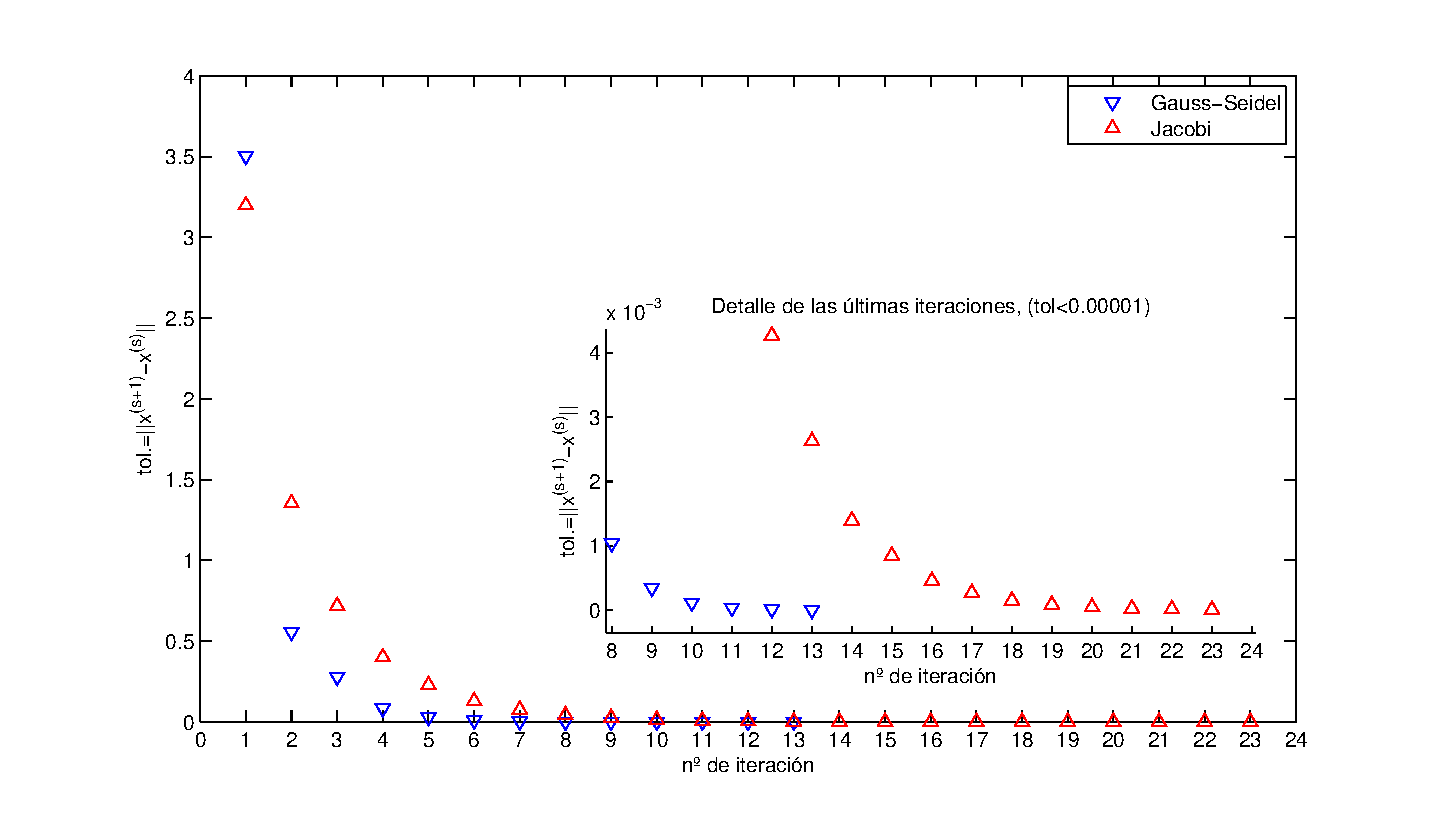
\includegraphics[width=16cm]{gjcom.eps}
\bicaption{evolución de la tolerancia (módulo de la diferencia entre dos soluciones sucesivas) para un mismo sistema resuelto mediante el método de Gauss-Seidel y el método de Jacobi}{evolution of the tolerance (modulus of the difference between two successive solutions) for the same system solved by the Gauss-Seidel method and the Jacobi method}
\label{fig:gjcom}
\end{figure}
\begin{paracol}{2}

\subsection{Amortiguamiento.} \index{Métodos amortiguados} El amortiguamiento consiste en modificar un método iterativo, de modo que en cada iteración, se da como solución la media ponderada de los resultados de dos iteraciones sucesivas,
\begin{equation*}
x^{(s+1)}=\omega \cdot x^{*}+(1-\omega) \cdot x^{(s)}
\end{equation*}

\switchcolumn
\subsection{Weighted methods.} \index{Weighted methods} In weighted iterations we  modify an iterative method so that at each iteration, the weighted average of the results of two successive iterations is given as the solution,
\begin{equation*}
x^{(s+1)}=\omega \cdot x^{*}+(1-\omega) \cdot x^{(s)}
\end{equation*}

\switchcolumn

Donde $x^{(*)}$ representa el valor que se obtendría aplicando una iteración del método a $x^{(s)}$, es decir sería el valor de $x^{(s+1)}$ si no se aplica amortiguamiento.

El parámetro $\omega$ recibe el nombre de factor de relajamiento. Si $0<\omega<1$ se trata de un método de subrelajación. Su uso permite resolver sistemas que no convergen si se usa el mismo método sin relajación. Si $\omega>1$ el método se llama de sobrerelajación, permite acelerar la convergencia respecto al mismo método sin relajación. Por último, si hacemos $\omega=1$, recuperamos el método original sin relajación.

\switchcolumn
Where $x^{(*)}$ represents the value that would be obtained by applying one iteration of the method to $x^{(s)}$, i.e. it would be the value of $x^{(s+1)}$ if no weight were applied.

The parameter $\omega$ is called the relaxation factor. If $$0<\omega<1$$ this is a method of under-relaxation. Its use makes it possible to solve systems that do not converge if the same method is used without relaxation. If $\omega>1$ the method is called over-relaxation, it allows to accelerate the convergence with respect to the same method without relaxation. Finally, if we make $\omegaº=1$, we recover the original method without relaxation.

\switchcolumn

\paragraph{El método de Jacobi amortiguado.} \index{Método de Jacobi amortiguado} Se obtiene aplicando el método de relajación que acabamos de describir, al método de Jacobi. La expresión general de una iteración del método de Jacobi amortiguando sería,

\switchcolumn
\paragraph{The weighted Jacobi method.} \index{Weighted Jacobi method}This is obtained by applying the relaxation method just described to Jacobi's method. The general expression for an iteration of the damped Jacobi method would be,
\end{paracol}

\begin{equation*}
x_i^{(s+1)}=\omega\cdot \overbrace{\frac{b_i-\sum_{j\neq i}a_{ij}x_j^{(s)}}{a_{ii}}}^{x^{(*)}}+(1- \omega)\cdot x_i^{s}
\end{equation*}

\begin{paracol}{2}
    Para implementarlo, bastaría añadir al código del método de Jacobi una línea incluyendo el promedio entre las dos soluciones sucesivas,
    \switchcolumn
To implement it, it would be sufficient to add to the code of Jacobi's method a line including the average between the two successive solutions,
\end{paracol}

\begin{minted}{python}
    error= np.linalg.norm(xs1-xs)
    it=0
    while error>tol:
        # For all the equations
        xs1=b.copy()
        for i in range(nf):
            for j in range(i):
                xs1[i]-=A[i,j]*xs[j]

            for j in range(i+1,nf):
                xs1[i]-=A[i,j]*xs[j]
            xs1[i]=xs1[i]/A[i,i]
        # Weighted iteration
        xs1=w*xs1+(1-w)*xs
        error= np.linalg.norm(xs1-xs)
        xs=xs1.copy()
        it+=1
        if it>itmax:
            break
\end{minted}

\begin{paracol}{2}

En forma matricial, la expresión general del método de Jacobi amortiguado sería,
\switchcolumn
In matrix form, the general expression for the damped Jacobi method would be,
\end{paracol}
\begin{equation*}
x^{(s+1)}=\omega\cdot\overbrace{\left(D^{-1}\cdot b- D^{-1}\cdot\left(L+U\right)\cdot x^{(s)}\right)}^{x^{(*)}}+(1-w)x^{(s)}
\end{equation*}

\begin{paracol}{2}
Si reorganizamos esta expresión,
\switchcolumn
Reordering the expression,
\end{paracol}


\begin{equation*}
x^{(s+1)}=\omega\cdot D^{-1}\cdot b+ \left[(1-w)\cdot I - w\cdot  D^{-1}\cdot  \left(L+U \right)\right]\cdot x^{(s)}
\end{equation*}

\begin{paracol}{2}
Podemos identificar fácilmente el termino fijo, $f=\omega\cdot D^{-1}\cdot b$ y la matriz del método $H=\left((1-w)\cdot I - w\cdot  D^{-1}\cdot  \left(L+U \right)\right)$.

Para implementar el código del método de Jacobi amortiguado, debemos calcular la matriz identidad del tamaño de sistema y modificar las expresiones de $f$ y $H$,

\switchcolumn
We can easily identify the fixed term  $f=\omega\cdot D^{-1}\cdot b$ and the method matrix $H=\left((1-w)\cdot I - w\cdot  D^{-1}\cdot  \left(L+U \right)\right)$.

To implement the code of the damped Jacobi method, we must calculate the identity matrix of the system size and modify the expressions of $f$ and $H$,

\end{paracol}

\begin{minted}{python}
    [nf,nc]=np.shape(A)
    xs=x0.copy()
    xs1=b.copy()
    error= np.linalg.norm(xs1-xs)
    it=0
    D=np.diag(np.diag(A))
    U=np.triu(A)-D
    L=np.tril(A)-D
    invD=np.linalg.inv(D)
    I=np.eye(nf)
    f=w*(invD).dot(b)
    H=(1-w)*I-w*invD.dot(L+U)
    # First iteration
    xs1=f+H.dot(xs)
    error=np.linalg.norm(xs1-xs)
    it+=1
    '''From here would come the code needed to calculate the 
    successive iterations until the solution converges''

\end{minted}
\begin{paracol}{2}
\paragraph{El método SOR.} \index{Método SOR}El método SOR --\emph{Succesive OverRelaxation}-- se obtiene aplicando amortiguamiento al método de Gauss-Seidel. Aplicando el mismo razonamiento que el caso de Jacobi amortiguado, la expresión general para una iteración del método SOR es,
\switchcolumn
\paragraph{The SOR method}. \index{SOR method}The SOR method -- ‘successive over-relaxation’ -- is obtained by applying a weigth to the Gauss-Seidel method. Applying the same reasoning as the weighted Jacobi case, the general expression for an iteration of the SOR method is,
\end{paracol}

\begin{equation*}
x_i^{(s+1)}=\omega\cdot \overbrace{\frac{b_i-\sum_{j< i}a_{ij}x_j^{(s+1)}-\sum_{j> i}a_{ij}x_j^{(s)}}{a_{ii}}}^{x^{(*)}}+(1-\omega)\cdot x_i^{(s)}
\end{equation*}

\begin{paracol}{2}

Al igual que en el caso de Jacobi amortiguado, para implementar el método SOR es suficiente añadir una línea que calcule el promedio de dos soluciones sucesivas,
\switchcolumn
As in the case of the damped Jacobi, to implement the SOR method it is sufficient to add a line that calculates the average of two successive solutions,
\end{paracol}

\begin{minted}{python}
        # For all the equations
        xs1=b.copy()
        for i in range(nf):
            # For all the terms above x[i]
            for j in range(i):
                xs1[i]-=A[i,j]*xs1[j]
            #For all the terms below x[i]    
            for j in range(i+1,nf):
                xs1[i]-=A[i,j]*xs[j]
            xs1[i]=xs1[i]/A[i,i]
        xs1=w*xs1+(1-w)*xs
        error= np.linalg.norm(xs1-xs)
        xs=xs1.copy()
        it+=1
 
\end{minted}

\begin{paracol}{2}
En forma matricial la expresión para una iteración del método SOR sería,
\switchcolumn
In matrix form the expression for one iteration of the SOR method would be,
\end{paracol}
\begin{equation*}
x^{(s+1)}= \omega\cdot\overbrace{\left((D+L)^{-1}\cdot b-(D+L)^{-1}\cdot U\cdot x^{(s)}\right)}^{x^{(*)}}+(1-\omega)\cdot x^{(s)}
\end{equation*}
\begin{paracol}{2}

Y tras reordenar,

\switchcolumn
And after reordering,

\end{paracol}

\begin{equation*}
x^{(s+1)}= \omega\cdot\left((D+L)^{-1}\cdot b\right)+\left[(1-\omega)\cdot I-\omega\cdot(D+L)^{-1}\cdot U\right]\cdot x^{(s)}
\end{equation*}

\begin{paracol}{2}
De nuevo, podemos identificar, el término fijo, $f=\omega\cdot\left((D+L)^{-1}\cdot b\right)$ y la matriz del método, $H=\left((1-\omega)\cdot I-\omega\cdot(D+L)^{-1}\cdot U\right)$.

El siguiente fragmento de código muestra la obtención de $f$ y $H$ para el método SOR,

\switchcolumn

Again, we can identify the fixed term, $f=\omega\cdot\left((D+L)^{-1}\cdot b\right)$ and the method matrix, $H=\left((1-\omega)\cdot I-\omega\cdot(D+L)^{-1}\cdot U\right)$.

The following code fragment shows how $f$ and $H$ are obtained for the SOR method,    
\end{paracol}

\begin{minted}{python}
    [nf,nc]=np.shape(A)
    xs=x0.copy()
    xs1=b.copy()
    error= np.linalg.norm(xs1-xs)
    it=0
    D=np.diag(np.diag(A))
    U=np.triu(A)-D
    L=np.tril(A)-D
    invD=np.linalg.inv(D+L)
    I=np.eye(nf)
    f=w*(invD).dot(b)
    H=(1-w)*I-w*invD.dot(U)
    #First iteration
    xs1=f+H.dot(xs)
    error=np.linalg.norm(xs1-xs)
    it+=1
    xs=xs1.copy()
    
\end{minted}

\begin{paracol}{2}
\subsection{Análisis de convergencia}\index{Análisis de convergencia}
En la introducción a los métodos iterativos dejamos abierta la cuestión de su convergencia. Vamos a analizar en más detalle en qué condiciones podemos asegurar que un método iterativo, aplicado a un sistema de ecuaciones lineales concreto, converge. 

En primer lugar, tenemos que definir qué entendemos por convergencia. Cuando un método iterativo converge, lo hace en forma asintótica. Es decir, haría falta un número infinito de iteraciones para alcanzar la solución exacta.

\begin{equation*}
x^{(0)}\rightarrow x^{(1)} \rightarrow x^{(2)}\rightarrow \cdots \rightarrow x^{(\infty)}=x
\end{equation*}

\switchcolumn

\subsection{Convergence analysis}\index{Convergence analysis}
In the introduction to iterative methods we left open the question of their convergence. Let us analyse in more detail under what conditions we can ensure that an iterative method, applied to a particular system of linear equations, converges. 

First of all, we have to define what we mean by convergence. When an iterative method converges, it does so asymptotically. That is, it would take an infinite number of iterations to reach the exact solution.

\begin{equation*}
x^{(0)}\rightarrow x^{(1)} \rightarrow x^{(2)}\rightarrow \cdots \rightarrow x^{(\infty)}=x
\end{equation*}

\switchcolumn

Lógicamente, es inviable realizar un número infinito de iteraciones. Por esta razón, las soluciones de los métodos iterativos son siempre aproximadas; realizamos un número finito de iteraciones hasta cumplir una determinada condición de convergencia. Como no conocemos la solución exacta, imponemos dicha condición entre dos iteraciones sucesivas,

\begin{equation*}
 \lVert x^{(s+1)}-x^{(s)}\rVert \leq C \Rightarrow  \lVert x^{(s+1)}-x\rVert = \lvert e^{(s+1)} \rvert
\end{equation*}

\switchcolumn
Logically, it is unfeasible to perform an infinite number of iterations. For this reason, the solutions of iterative methods are always approximate; we perform a finite number of iterations until a certain convergence condition is met. Since we do not know the exact solution, we impose this condition between two successive iterations,

\begin{equation*}
 \lVert x^{(s+1)}-x^{(s)}\rVert \leq C \Rightarrow  \lVert x^{(s+1)}-x\rVert = \lvert e^{(s+1)} \rvert
\end{equation*}

\switchcolumn
Donde $e^{(s+1)}$ representaría el error \emph{real} de convergencia cometido en la iteración $s+1$.

Tomando como punto de partida la expresión general del cálculo de una iteración en forma matricial,
\begin{equation*}
x^{(s+1)}=f+H\cdot x^{(s)}
\end{equation*}

\switchcolumn
Where $e^{(s+1)}$ would represent the real convergence error committed in iteration $s+1$.

Taking as a starting point the general expression for the calculation of an iteration in matrix form,
\begin{equation*}
x^{(s+1)}=f+H\cdot x^{(s)}
\end{equation*}

\switchcolumn
Podemos expresar el error de convergencia como,
\begin{equation*}
e^{(s+1)}=x^{(s+1)}-x=f+H\cdot x^{(s)}-x
\end{equation*}

\switchcolumn
We can express the convergence error as,
\begin{equation*}
e^{(s+1)}=x^{(s+1)}-x=f+H\cdot x^{(s)}-x
\end{equation*}

\switchcolumn
Pero la solución exacta, si pudiera alcanzarse, cumpliría,

\begin{equation*}
x=f+H\cdot x
\end{equation*}

\switchcolumn

But the exact solution, if it could be achieved, would comply,
\begin{equation*}
x=f+H\cdot x
\end{equation*}

\switchcolumn
Y si sustituimos en la expresión del error de convergencia,

\begin{equation*}
e^{(s+1)}=f+H\cdot x^{(s)}-f-H\cdot x
\end{equation*}

\switchcolumn

And if we substitute in the expression for the convergence error,

\begin{equation*}
e^{(s+1)}=f+H\cdot x^{(s)}-f-H\cdot x
\end{equation*}

\switchcolumn

Llegamos finalmente a la siguiente expresión, que relaciona los errores de convergencia de dos iteraciones sucesivas,

\begin{equation*}
e^{(s+1)}=H\cdot e^{(s)}
\end{equation*}

\switchcolumn

We finally arrive to the following expression, that relates the convergence errors between two sucessive iterations,

\begin{equation*}
e^{(s+1)}=H\cdot e^{(s)}
\end{equation*}

\switchcolumn
Para que el error disminuya de iteración en iteración y el método converja, es necesario que la matriz del método $H$ tenga norma-2  menor que la unidad.

\switchcolumn
For the error to decrease from iteration to iteration and for the method to converge, the method matrix $H$ must have norm-2 less than unity.

\switchcolumn
Supongamos que un sistema de dimension $n$ su matriz del método $H$, tiene un conjunto de $n$ autovectores linealmente independientes, $w_1, \ w_2, \cdots, \ w_n$, cada uno asociado a su correspondiente autovalor, $\lambda_1, \ \lambda_2, \ \cdots,\ \lambda_n$. El error de convergencia, es también un vector de dimensión $n$, por tanto podemos expresarlo como una combinación lineal de los $n$ autovectores linealmente independientes de la matriz $H$. Supongamos que lo hacemos para el error de convergencia $e^{(0)}$ correspondiente al valor inicial de la solución $x^{(0)}$,

\switchcolumn
Suppose that a system of dimension $n$ its method matrix $H$, has a set of $n$ linearly independent eigenvectors, $w_1, w_2, \cdots, w_n$, each one associated to its corresponding eigenvalue, $\lambda_1, \lambda_2, \cdots, \lambda_n$. The convergence error is also a vector of dimension $n$, so we can express it as a linear combination of the $n$ linearly independent eigenvectors of the matrix $H$. Suppose we do this for the convergence error $e^{(0)}$ corresponding to the initial value of the solution $x^{(0)}$,
\end{paracol}

\begin{equation*}
e^{(0)}=\alpha_1\cdot w_1+\alpha_2\cdot w_2+\cdots+\alpha_n\cdot w_n
\end{equation*}

\begin{paracol}{2}
Si empleamos la ecuación deducida antes para la relación del error entre dos iteraciones sucesivas y recordando que aplicar una matriz a un autovector, es equivalente a multiplicarlo por el autovalor correspondientes: $H\cdot w_i=\lambda_i\cdot w_i$, obtenemos para el error de convergencia en la iteración $s$,

\switchcolumn
If we use the equation deduced earlier for the error ratio between two successive iterations and remembering that applying a matrix to an eigenvector is equivalent to multiplying it by the corresponding eigenvalue: $H\cdot w_i=\lambda_i\cdot w_i$, we obtain for the error of convergence at iteration $s$,
\end{paracol}



\begin{align*}
e^{(1)}&=H\cdot e^{(0)}=\alpha_1\cdot \lambda_1 \cdot  w_1+\alpha_2\cdot \lambda_2 \cdot  w_2+\cdots+\alpha_n\cdot \lambda_n \cdot w_n\\
e^{(2)}&=H\cdot e^{(1)}=H^2\cdot e^{(0)}=\alpha_1\cdot \lambda_1^2 \cdot  w_1+\alpha_2\cdot \lambda_2^2 \cdot  w_2+\cdots+\alpha_n\cdot \lambda_n^2 \cdot w_n\\
\vdots \ \ \ & \\
e^{(s)}&=H\cdot e^{(s-1)}=H^s\cdot e^{(0)}=\alpha_1\cdot \lambda_1^s \cdot  w_1+\alpha_2\cdot \lambda_2^s \cdot  w_2+\cdots+\alpha_n\cdot \lambda_n^s \cdot w_n
\end{align*}

\begin{paracol}{2}
Para que el error tienda a cero, $e^{(s)}\rightarrow 0$ al aumentar $s$, para cualquier combinación inicial de valores $\alpha_i$, esto es para cualquier aproximación inicial $x^{(0)}$, es necesario que todos los autovalores de la matriz del método cumplan,

\begin{equation*}
\vert \lambda_i \vert < 1
\end{equation*}

\switchcolumn
For the error to tend to zero, $e^{(s)}\rightarrow 0$ as $s$ increases, for any initial combination of values $\alpha_i$, i.e. for any initial approximation $x^{(0)}$, it is necessary that all the eigenvalues of the method matrix satisfy,

\begin{equation*}
\vert \lambda_i \vert < 1
\end{equation*}

\switchcolumn

Por tanto, el sistema converge si el radio espectral de la matriz del método es menor que la unidad. \footnote{El radio espectral de una matriz es el mayor de sus autovalores en valor absoluto.}

\begin{equation*}
\rho(H)<1 \Rightarrow \lim_{s\rightarrow \infty}e^{(s)}=0
\end{equation*}

\switchcolumn
Therefore, the system converges if the spectral radius of the method matrix is less than unity. \footnote{The spectral radius of a matrix is the largest of its eigenvalues in absolute value.}

\begin{equation*}
\rho(H)<1 \Rightarrow \lim_{s\rightarrow \infty}e^{(s)}=0
\end{equation*}

\end{paracol}

\begin{paracol}{2}
\paragraph{Velocidad de convergencia.} \index{Velocidad de convergencia}Para un número de iteraciones suficientemente grande, el radio espectral de la matriz del método nos da la velocidad de convergencia. Esto es debido a que el resto de los términos del error, asociados a otros autovalores más pequeños tienden a cero más  deprisa. Por tanto podemos hacer la siguiente aproximación, donde estamos suponiendo que el autovalor $\lambda_n$ es el radio espectral,

\switchcolumn
\paragraph{Speed of convergence}. \index{Speed of convergence}For a sufficiently large number of iterations, the spectral radius of the method matrix gives the speed of convergence. This is because the remaining error terms associated with other smaller eigenvalues tend to zero faster. We can therefore make the following approximation, where we are assuming that the eigenvalue $\lambda_n$ is the spectral radius,
\end{paracol}

\begin{equation*}
e^{(s)}\approx c_n \rho(H)^s w_n= c_n \lambda_n^s w_n
\end{equation*}

\begin{paracol}{2}

Podemos ahora calcular cuantas iteraciones nos costará reducir un error inicial por debajo de un determinado valor. Esto dependerá de la solución inicial y de radio espectral de la matriz del método,

\switchcolumn
We can now calculate how many iterations it will take to reduce an initial error below a certain value. This will depend on the initial solution and the spectral radius of the method matrix,

\end{paracol}

\begin{equation*}
e^{(s)}\approx  \rho(H)^s e^{(0)} \Rightarrow \frac{e^{(s)}}{e^{(0)}} \approx \rho(H)^s
\end{equation*}

\begin{paracol}{2}
así por ejemplo si queremos reducir el error inicial en $m$ dígitos,
\switchcolumn
so for example if we want to reduce the initial error by $m$ digits,
\end{paracol}

\begin{equation*}
\frac{e^{(s)}}{e^{(0)}} \approx \rho(h)^s \leq 10^{-m} \Rightarrow s \geq \frac{-m}{\log_{10}\left(\rho(H)\right)}
\end{equation*}

\begin{paracol}{2}
La matriz del método juega por tanto un papel fundamental tanto en la convergencia del método, como en la velocidad (número de iteraciones) con la que el método converge. Los métodos amortiguados, permiten modificar la matriz de convergencia, gracias al factor de amortiguamiento $\omega$, haciendo que sistemas para los que no es posible encontrar una solución mediante un método iterativo converjan.

Como ejemplo, el sistema,

\switchcolumn
The method matrix therefore plays a fundamental role both in the convergence of the method and in the speed (number of iterations) with which the method converges. Damped methods allow the convergence matrix to be modified, thanks to the damping factor $omega$, making systems for which it is not possible to find a solution by means of an iterative method converge.

As an example, the system,
\end{paracol}

\begin{equation*}
\begin{pmatrix}
1& 2& -1\\
2& -5& 1\\
1& -1& 3
\end{pmatrix}\cdot \begin{pmatrix}
x_1\\
x_2\\
x_3
\end{pmatrix}=\begin{pmatrix}
2\\
-5\\
8
\end{pmatrix}
\end{equation*}

\begin{paracol}{2}
No converge si tratamos de resolverlo por el método de Jacobi. Sin embargo si es posible obtener su solución empleando el método de Jacobi Amortiguado. La figura \ref{fig:cjjam}  muestra la evolución de la tolerancia para dicho sistema empleando ambos métodos.
\switchcolumn
It does not converge if we try to solve it by the Jacobi method. However, it is possible to obtain its solution using the Weighted Jacobi method. Figure \ref{fig:cjjam} shows the evolution of the tolerance for this system using both methods.
\end{paracol}

\begin{figure}[h]
\centering
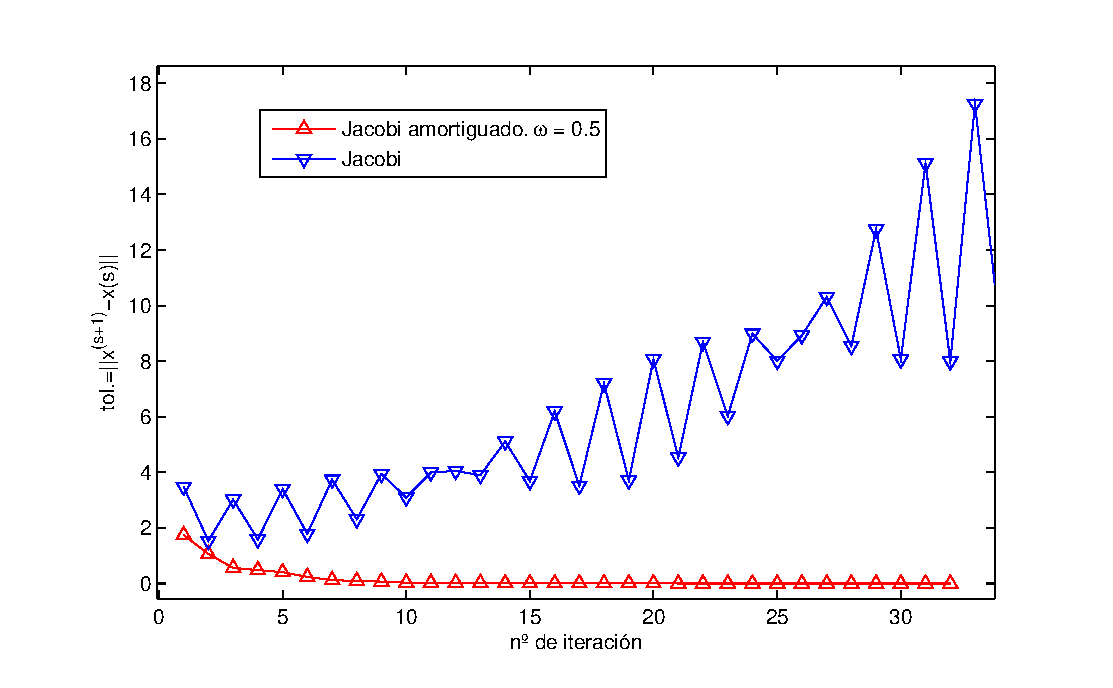
\includegraphics[width=14cm]{comjjam.eps}
\bicaption{Evolución de la tolerancia para un mismo sistema empleando el metodo de Jacobi (diverge) y el de Jacobi amortiguado (converge).}{Tolerance evolution for the same system using the Jacobi method (diverges) and the weighted Jacobi method (converges).}
\label{fig:cjjam}


\end{figure}

\begin{paracol}{2}
Si calculamos el radio espectral de la matriz del método, para el método de Jacobi tendríamos,
\switchcolumn
If we calculate the spectral radius of the method matrix, for the Jacobi method we would have,

\end{paracol}

\begin{minted}{python}
import numpy as np
A=np.array([[1,2,-1],[2,-5,1],[1,-1,3]])
D=np.diag(np.diag(A))
U=np.triu(A)-D
L=np.tril(A)-D
invD=np.linalg.inv(D)
H=invD.dot(L+U)
eigenvalues,eigenvectors=np.linalg.eig(H)
spectral_rad=np.max(np.abs(eigenvalues))
print("Eigenvalues: ",eigenvalues)
print("Spectral radius: ", spectral_rad)
\end{minted}

\begin{minted}{pycon}
Eigenvalues:  [ 0.11872445+1.05306845j  0.11872445-1.05306845j -0.2374489 +0.j        ]
Spectral radius:  1.0597398959658624
\end{minted}

\begin{paracol}{2}
El radio espectral es mayor que la unidad y el método no converge.

Si repetimos el cálculo para el método de Jacobi amortiguado, con $\omega=0.5$

\switchcolumn
The spectral radius is greater than unity and the method does not converge.

If we repeat the calculation for the weighted Jacobi method, with $\omega=0.5$,
\end{paracol}

\begin{minted}{python}
D=np.diag(np.diag(A))
U=np.triu(A)-D
L=np.tril(A)-D
invD=np.linalg.inv(D)
w=0.5
I=np.eye(3)
H=(1-w)*I-w*invD.dot(L+U)
eigenvalues,eigenvectors=np.linalg.eig(H)
spectral_rad=np.max(np.abs(eigenvalues))
print("Eigenvalues: ",eigenvalues)
print("Spectral radius: ", spectral_rad)

\end{minted}

\begin{minted}{pycon}
Eigenvalues:  [0.44063777+0.52653422j 0.44063777-0.52653422j 0.61872445+0.j        ]
Spectral radius:  0.6865857095839855
\end{minted}

\begin{paracol}{2}

El radio espectral es ahora menor que la unidad y el método converge.

Por último indicar que cualquiera de los métodos iterativos descrito converge para un sistema que cumpla que su matriz de coeficientes es estrictamente diagonal dominante.

\switchcolumn
The spectral radius is now smaller than unity and the method converges.

Finally, it should be noted that any of the iterative methods described converges for a system whose coefficient matrix is strictly diagonally dominant.

\end{paracol}
\section{Ejercicios}
\begin{enumerate}
\item Crea una función en python que calcule la solución de un sistema de ecuaciones triangular inferior empleando el método de sustituciones progresivas. La función deberá tomar como valores de entrada una matriz triangular inferior de dimensión $(n\times n)$ arbitraria y un vector columna $(n\times 1)$ de términos independientes. Deberá devolver como variable de salida un vector columna $(n\times 1)$ con las soluciones del sistema.

\item \label{eje62} Crea una función en python que calcule la solución de un sistema de ecuaciones triangular superior empleando el método de sustituciones regresivas. La función deberá tomar como valores de entrada una matriz triangular inferior de dimensión $(n\times n)$ arbitraria y un vector columna $(n\times 1)$ de términos independientes. Deberá devolver un vector columna $(n\times 1)$ con las soluciones del sistema.

\item Crea una función que dadas una matriz cuadrada  $ A,\ (n\times n)$ y un  vector columna $b,\ (n\times 1)$, construya la matriz ampliada $Ab$, Aplique el método de eliminación gausiana a la matriz ampliada y llame a la función creada en el ejercicio \ref{eje62} Para resolver el sistema $Ax=b$. La función deberá devolver como variables de salida, La matriz resultante de la aplicar la eliminación gaussiana a la ampliada y un vector columna con las soluciones del sistema resuelto. 

\item Crea una función que dadas una matriz cuadrada  $ A,\ (n\times n)$ y un  vector columna $b,\ (n\times 1)$, construya la matriz ampliada $Ab$. Aplique el método de eliminación Gauss-Jordan a la matriz ampliada y devuelva como variable de salida la matriz en forma escalonada reducida por filas, de modo que la última fila sea la solución del sistema $Ax=b$  

\item Construye un programa que resuelva un sistema de ecuaciones de dimensión arbitraria, empleando el método de Jacobi simple (no en forma matricial). El programa deberá admitir como variables de entrada, una matriz de coeficientes $ A,\ (n\times n)$, un vector de términos independientes $b,\ (n\times 1)$, una solución inicial $x_0 ,\ (n\times 1)$, un valor para la tolerancia máxima entre dos iteraciones sucesivas y un número máximo de iteraciones permitido. El programa deberá devolver un vector columna con las soluciones del sistema, el número de iteraciones empleado y el error relativo entre las dos últimas iteraciones realizadas.

\item Repite el ejercicio anterior empleando ahora el método de Jacobi matricial. Añade el código necesario para que calcule en primer lugar el radio espectral de la matriz del método y caso de no cumplirse  la condición de convergencia, el programa interrumpa su ejecución y devuelva un mensaje de error indicando el valor del radio espectral.

\item Construye un programa que resuelva un sistema de ecuaciones de dimensión arbitraria, empleando el método de Gauss-Seidel simple (no en forma matricial). El programa deberá admitir como variables de entrada, una matriz de coeficientes $ A,\ (n\times n)$, un vector de términos independientes $b,\ (n\times 1)$, una solución inicial $x_0 ,\ (n\times 1)$, un valor para la tolerancia máxima entre dos iteraciones sucesivas y un número máximo de iteraciones permitido. El programa deberá devolver un vector columna con las soluciones del sistema, el número de iteraciones empleado y el error relativo entre las dos últimas iteraciones realizadas.

\item Repite el ejercicio anterior empleando ahora el método de Gauss-Seidel matricial. Añade el código necesario para que calcule en primer lugar el radio espectral de la matriz del método y caso de no cumplirse  la condición de convergencia, el programa interrumpa su ejecución y devuelva un mensaje de error indicando el valor del radio espectral.

\item Construye un programa que resuelva un sistema de ecuaciones de dimensión arbitraria, empleando el método de Jacobi amortiguado simple (no en forma matricial). El programa deberá admitir como variables de entrada, una matriz de coeficientes $ A,\ (n\times n)$, un vector de términos independientes $b,\ (n\times 1)$, una solución inicial $x_0 ,\ (n\times 1)$, un valor para el parámetro de amortiguamiento $\omega$, un valor para la tolerancia máxima entre dos iteraciones sucesivas y un número máximo de iteraciones permitido. El programa deberá devolver un vector columna con las soluciones del sistema, el número de iteraciones empleado y el error relativo entre las dos últimas iteraciones realizadas.

\item Repite el ejercicio anterior empleando ahora el método de Jacobi amortiguado matricial. Añade el código necesario para que calcule en primer lugar el radio espectral de la matriz del método y caso de no cumplirse  la condición de convergencia, el programa interrumpa su ejecución y devuelva un mensaje de error indicando el valor del radio espectral.

\item Construye un programa que resuelva un sistema de ecuaciones de dimensión arbitraria, empleando el método SOR  simple (no en forma matricial). El programa deberá admitir como variables de entrada, una matriz de coeficientes $ A,\ (n\times n)$, un vector de términos independientes $b,\ (n\times 1)$, una solución inicial $x_0 ,\ (n\times 1)$, un valor para el parámetro de amortiguamiento $\omega$, un valor para la tolerancia máxima entre dos iteraciones sucesivas y un número máximo de iteraciones permitido. El programa deberá devolver un vector columna con las soluciones del sistema, el número de iteraciones empleado y el error relativo entre las dos últimas iteraciones realizadas.

\item Repite el ejercicio anterior empleando ahora el método SOR matricial. Añade el código necesario para que calcule en primer lugar el radio espectral de la matriz del método y caso de no cumplirse  la condición de convergencia, el programa interrumpa su ejecución y devuelva un mensaje de error indicando el valor del radio espectral.


\item Resuelve el siguiente sistema de ecuaciones, empleando la factorización LU. Indica todos los pasos empleados hasta obtener las solución del sistema.
\begin{align*}
3x_1&+3x_2-2x_3 +\ x_4= 13\\
 &+2x_2-\ x_3  \hspace{30pt} =\ 3\\
-2x_1&+\ x_2 + 5x_3 -4x_4=\ 1\\
2x_1& \hspace{30pt} -\ x_3 +2x_4 =\ 5
\end{align*}
Repite el ejercicio empleando las factorizaciones QR y SVD.

\item Para calcular las intensidades de un circuito de corriente continua como el de la figura, es suficiente emplear las leyes de Kirchoff. La primera ley --\emph{ley de nodos}-- establece que la suma de corrientes que llegan a un nodo del circuito debe ser igual a cero.
La segunda --\emph{ley de mallas}-- establece que la suma de las caídas de tensión en un malla cerrada tiene que ser cero. La caída de voltaje en una resistencia se calcula empleando la ley de Ohm: $V = i\cdot R$
Si aplicamos las leyes de Kirchoff al circuito de la figura, obtenemos  el siguiente sistema de ecuaciones,

\begin{minipage}{0.3\textwidth}
\begin{align*}
i_1 - i_2 - i_3 &= 0\\
i_3 - i_4 - i_5 &= 0\\
i_5  + i_2 -i_6&= 0\\
5i_3 + 70 i_4 &= 180\\
25i_2 -5i_3-10i_5 &= 0\\
10i_5+8i_6 -70i_4 &= 0  
\end{align*}
\end{minipage}
\begin{minipage}{0.7\textwidth}
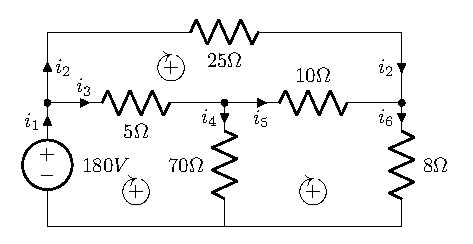
\includegraphics[scale=1.1]{circuito.eps}
\end{minipage}
\ \\
Las tres primeras ecuaciones corresponden a aplicar la \emph{ley de nodos} a los nodos marcados con un punto negro en la figura. 

Las tres últimas, a aplicar la \emph{ley de mallas} a las tres mallas considerando positivo recorrerlas en el sentido de las agujas del reloj.

El sistema de ecuaciones obtenido puede expresarse en forma matricial como,
\begin{equation}\label{cucu}
\begin{pmatrix}
1& -1& -1& 0 & 0 &0\\
0& 0& 1& -1& -1& 0\\
0& 1& 0&  0&  1& -1\\ 
0& 0& 5& 70& 0& 0\\
0& 25& -5& 0& -10& 0\\
0& 0& 0& -70& 10& 8
\end{pmatrix}\begin{pmatrix}
i_1\\ i_2\\ i_3\\ i_4\\ i_5\\ i_6
\end{pmatrix}= \begin{pmatrix}
0\\ 0\\ 0\\ 180\\ 0\\ 0
\end{pmatrix} 
\end{equation}



\begin{enumerate}
\item Define en python el sistema de ecuaciones (\ref{cucu}). Obtén los valores de las intensidades en todas las ramas del circuito empleando directamente un solo comando o función de python. Calcula el condicionamiento del sustema y dí si en tu opinión el sistema está bien o mal condicionado.

\item Emplea la factorización QR para obtener de nuevo la solución del sistema. 

\item Utilizando la versión permutada del sistema, obtenida mediante la factorización LU, es decir, usando $P\cdot A$ como matriz del sistema y $P\cdot b$, como término independiente, calcula el radio espectral correspondiente al método de Jacobi e indica si tiene sentido o no emplear este método para obtener las intensidades del circuito de la figura.

\item Emplea el método de Jacobi amortiguado, con un amortiguamiento de $\omega =0.1$ para calcular las intensidades del circuito de la figura, con una tolerancia de $10^{-5}$. Indica el número de iteraciones empleado hasta alcanzar la solución.  (\emph{Nota importante:} Usa la versión permutada del sistema y ten en cuenta que va a necesitar bastantes iteraciones --más de $3000$-- para converger).

\item Emplea el método SOR, con un amortiguamiento de $\omega =0.2$ para calcular las intensidades del circuito de la figura, con una tolerancia de $10^{-5}$. Indica el número de iteraciones empleado hasta alcanzar la solución (\emph{Nota importante:} Usa la versión permutada del sistema).
Discute, a la vista de los resultados, cúal método funciona mejor.

\item Escribe un código que permita dibujar el radio espectral de un método amortiguado en función de la matriz del método, para distintos valores del amortiguamiento. Emplea el programa para los casos de las dos preguntas anteriores. ¿Ha sido razonable la elección de los valores de $\omega$ realizada en dichas preguntas?
\end{enumerate}
\end{enumerate}

\section{Test del curso 2020/21}
\noindent \textbf{Problema 1}. El método iterativo de Richardson para la resolución de sistemas de ecuaciones lineales emplea la siguiente fórmula de recurrencia
\begin{equation}\label{eq:1}
x^{(s+1)} = x^{(s)} + \omega\left( b - Ax^{(s)}\right),
\end{equation}  
		donde $A \in \mathbb{R}^{n\times n}$ y $b  \in \mathbb{R}^{n}$ representan respectivamente la matriz de coeficientes y el vector columna de términos independientes del sistema de ecuaciones $Ax=b$ de orden $n\in\mathbb{N}$, y $x^{(s)}\in\mathbb{R}^n$ es el vector solución en la iteración $s\in\mathbb{N}$. El parámetro $\omega \in \mathbb{R}$  juega el mismo papel que el factor de relajación en los métodos amortiguados y debe ajustarse para asegurar la convergencia del método.

 \begin{enumerate}
\item {\bf 1 punto.} Reescribe la fórmula de recurrencia del método Richardson (ecuación \ref{eq:1})  en la forma matricial estándar
\begin{equation}\label{eq:2}
x^{(s+1)} = f + Hx^{(s)}.
\end{equation}

\item {\bf 2 puntos.} Construye una función en python que implemente el método de Richardson enpleando la forma matricial estándar, es decir, en cada iteración aplicamos la ecuación (\ref{eq:2}). La función deberá tomar como variables de entrada: 
\begin{enumerate}
	\item La matriz de coeficientes $A$.
	\item El vector de términos independientes $b$.
	\item El valor inicial $x^{(0)}$.
	\item Número máximo de iteraciones a realizar.
	\item Tolerancia mínima para el error entre iteraciones sucesivas.
	\item Un valor para el parámetro $\omega$.
\end{enumerate}
Así mismo, la función deberá devolver como variables de salida: 
\begin{enumerate}
\item La solución del sistema.
\item La tolerancia alcanzada.
\item El número de iteraciones empleado en obtener la solución.
\end{enumerate}

\item {\bf 2 puntos.} Emplea los métodos de Richardson, Jacobi y Gauss-Seidel para obtener la solución del sistema de ecuaciones
\begin{equation*}
\begin{pmatrix}
5&2&3&-1\\
2&6&3&0\\
1&-4&4&-1\\
2&0&3&7
\end{pmatrix}\begin{pmatrix}
x_1\\ x_2\\ x_3\\ x_4
\end{pmatrix}= \begin{pmatrix}
14\\ 23\\1\\ 39
\end{pmatrix}.
\end{equation*}
		 Emplea un valor $\omega = 0.16$ para el método de Richardson y una tolerancia de $10^{-5}$ para los tres métodos. Escoge el valor $x^{(0)}=\left[0,0,0,0\right]^T$ para los tres métodos.

Clasifica los tres métodos de mejor a peor, tomando como criterio el número de iteraciones empleado por cada uno de ellos para alcanzar la solución.

% \item {\bf 2 puntos.} \textcolor{red}{Define el error de la solución propuesta en la iteración $s$ con respecto al valor real de la solución $x$, esto es, $e^{(s)} = x^{(s)} - x$. Halla la matriz $W\in\mathbb{R}^{n\times n}$ que satisface:}
%	\begin{equation}
%		e^{(s+1)} = We^{(s)}.
%		\label{eq: error}
%	\end{equation}
%	 Metodología/pista: Sustituye $x^{(s)} = e^{(s)} + x$ en (\ref{eq:1}), y opera hasta alcanzar (\ref{eq: error}).

\item {\bf 2 punto.} Haz una gráfica del radio espectral de $H$ en función del parámetro $\omega$ para el método de Richardson y el sistema de ecuaciones del apartado anterior. Emplea para ello valores de $\omega$ comprendidos en el intervalo $[0.01\ 0.9]$, toma una separación entre valores de $0.01$.  Representa cada valor como un punto independiente.

Determina, a la vista de la gráfica, si sería posible encontrar un valor de $\omega$ para el que se alcance la solución del sistema en menos iteraciones, manteniendo la misma tolerancia. Indica, también de acuerdo con el gráfico, cuál es mayor valor de $\omega$ admisible. Razona las respuestas.
\end{enumerate}

\noindent \textbf{Problema 2.} El método de Gauss-Jordan permite resolver sistemas de ecuaciones lineales de la forma $Ax =b, A \in \mathbb{R}^{n\times n}$ y $x,b  \in \mathbb{R}^{n}$. Si en lugar de emplear un vector columna de términos independientes, sustituimos $b$ por una matriz $B$ de dimensión $n\times m$, el método nos permite obtener como resultado una matriz de soluciones $X$ también de dimension  $n\times m$: $AX=B$. Cada columna, $x_j, \, j\in\{1,\dots,m\}$, de la matriz $X$ representa la solución de sistema $Ax_j=b_j$, donde $b_j$ es la columna correspondiente de la matriz $B$. Es decir: hemos resuelto $m$ sistemas de ecuaciones simultáneamente.

\begin{enumerate}
\item {\bf 2 puntos.} Emplea el método de Gauss-Jordan para obtener la solución de $AX=B$, donde $A$ es la matriz de coeficientes del Problema 1 y B es la matriz identidad de dimension $4\times4$.
\item {\bf 1 punto.} ¿Sabrías decir que relación hay entre las matrices X y A?
\end{enumerate}



